	\chapter{Results}\label{cha:results}
	
		\section{1D geological reservoir model results}
	
c			\subsection{Scoring}
			\begin{figure}[h]
				\centering
				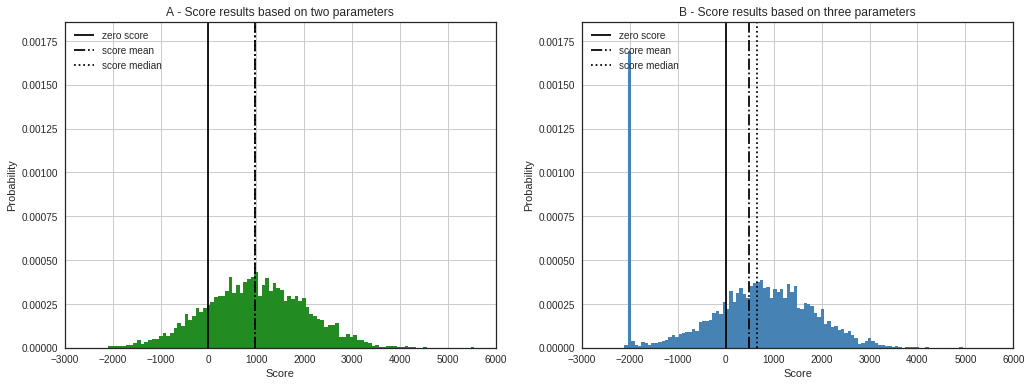
\includegraphics[width=1\textwidth]{Figures/score_results1.png}
				\caption{Posterior probability distributions from modeling scores using two (A) and three parameters (B) (reservoir thickness, reservoir top depth and seal thickness with a safety threshold of 20~m).}\label{fig:score_results1}
			\end{figure}
			Results from scoring based on simple Monte Carlo error propagation (10000 iterations) using only the priors of the 1D model (as defined in Section \ref{sec:1D_construction}) are plotted in Figure \ref{fig:score_results1}. A test run of scoring with only the two parameters reservoir thickness and depth, is shown in Figure \ref{fig:score_results1} (A). These results are represented by an approximately normal distribution. The score is negative in about 17\% of the cases. Mean and median are about the same.\\	
			Full scoring results, including also seal reliability (with a threshold of 20~m) as a parameter, are visualized in Figure \ref{fig:score_results1} (B). The main distribution is not changed significantly, except for a striking peak of probability at the possibility for a score of -2000. This presumably represents the bulk of cases in which the seal is assumed to have failed. Regarding this, it is to be noted, that the mean of the seal top distribution is found at -2000 m. It can be seen in Figure \ref{fig:update_moderate1} (A1), that around that depth in the model column, reservoir top and seal top probability distributions significantly overlap. Thus, there is a possibility for a higher score, due to a shallower reservoir top position, but also a high probability for a seal thickness below the safety cut-off threshold of 20~m. The negative score peak at -2000 is thus presumably caused by a high number of seal failures, due to both layer interfaces located within this range. Furthermore, as a consequence of this negative peak, mean and median of the score distribution have been shifted to lower values and are now found further apart (see Figure \ref{fig:score_results1} (B)).\\
			Using this prior score distribution as a base, the custom loss function including risk was applied (see Figure \ref{fig:1D_LFR}). It can be observed that the minima for expected loss, i.e. the Bayesian estimators for differently risk-affine actors, are located at different estimates. Mean and median of the score distribution are clearly surpassed by the best estimate of the most risk-friendly actor (\textit{r} = 0.5), while for the most risk-averse actors (\textit{r} = 1.25 and \textit{r} = 1.5), the Bayes action equals a zero score estimate and thus the decision to take no action. It can also be recognized that the expected loss is generally lower for risk-friendlier actors on the side of positive estimates, which in this case is the relevant side for decision-making.		
			%\subsection{Applying the custom loss function on the 1D reservoir scores}
			%\begin{figure}[p!]
			%	\centering
			%	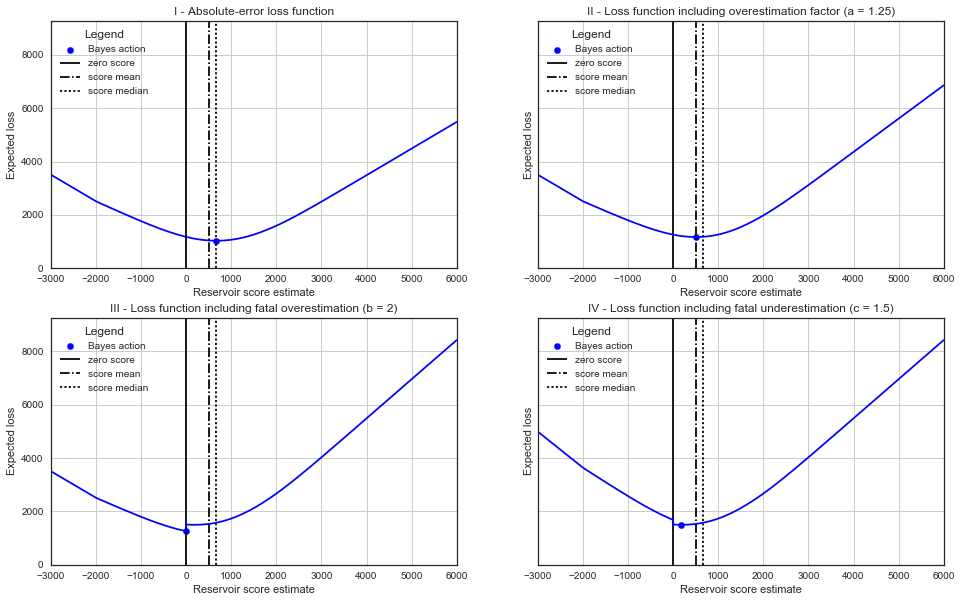
\includegraphics[width=1\textwidth]{Figures/LF_4steps.png}
			%	\caption{The single steps of customizing the loss function are depicted in plots I to IV.}\label{fig:LF_4steps}
			%\end{figure}			
			\begin{figure}[h]
				\centering
				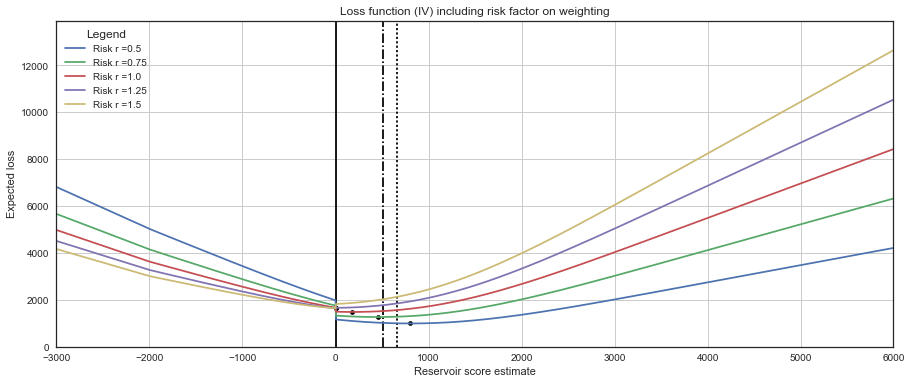
\includegraphics[width=1\textwidth]{Figures/LFR.png}
				\caption{Plotting of expected loss realizations after including the risk factor $r$ in the loss function  for actors with risk-affinities ranging from risk-averse ($r$ = 0.5 and 0.75), over risk-neutral ($r$ = 1), to risk-friendly ($r$ = 1.25 and $r$ = 1.5), based on the application of the custom loss function (Equation \ref{eq:LFR_final}) on a prior score distribution (see Figure \ref{fig:score_results1} (B)) from simple Monte Carlo error propagation.}\label{fig:1D_LFR} 
			\end{figure}			
			%Realizations of the four loss function adaption steps as elaborated in Section \ref{sec:LF_design} and based on the scoring results shown in Figure \ref{fig:score_results1}-B are depicted in the plots in Figure \ref{fig:LF_4steps}.
			%As expected, the median is returned for the Bayes action, when using the standard symmetric absolute-error loss function (Figure \ref{fig:LF_4steps}-I). Compared to this, it can be observed that assigning a stronger weight on overestimation (Figure \ref{fig:LF_4steps}-II) steepens the curve on the right hand side and shifts the minimum to the left, i.e. to a lower estimate. Using \textit{a} = 1.25, the Bayes action changes from the median, to a value close to the mean of the distribution. The shift and steepening are significantly reinforced by the introduction of fatal overestimation (Figure \ref{fig:LF_4steps}-III). With \textit{b} = 2, the Bayes action drops to the zero score estimate. It can also be noted, that by defining a condition dependent on the algebraic sign of the values, according to which only losses for positive estimates are multiplied by \textit{b}, a distinct jump appears at the zero score boundary. Due to a similar condition, the same effect is observed on the negative side of estimate values, where the curve has also been steepened, after including fatal underestimation (Figure \ref{fig:LF_4steps}-IV). This comes with a shift of the minimum towards positive values. It is also to be noted that with every customization step, the overall expected loss is increased.\\			
			%The implementation of the final custom loss function (Figure \ref{fig:LF_4steps}-IV) using single determined values for the true score is plotted in Figure \ref{fig:LF4_det_values}. This helps to clarify the way real losses result for each guess, relative to given true score values. The expected loss is acquired by arithmetically averaging such loss realizations based on the true score probability distribution by using Equation \ref{eq:ExpectedLoss2}.\\			
			%Implementing risk-affinity as a factor \textit{r} leads to different steepnesses of the plotted curves depicting loss and expected loss. The effect on the latter is visualized in Figure \ref{fig:1D_LFR}, where 0.5, 0.75, 1, 1.25 and 1.5 were chosen as values for \textit{r}. 

			\subsection{Bayesian inference using thickness likelihood functions}	
			\begin{figure}[p!]
				\centering
				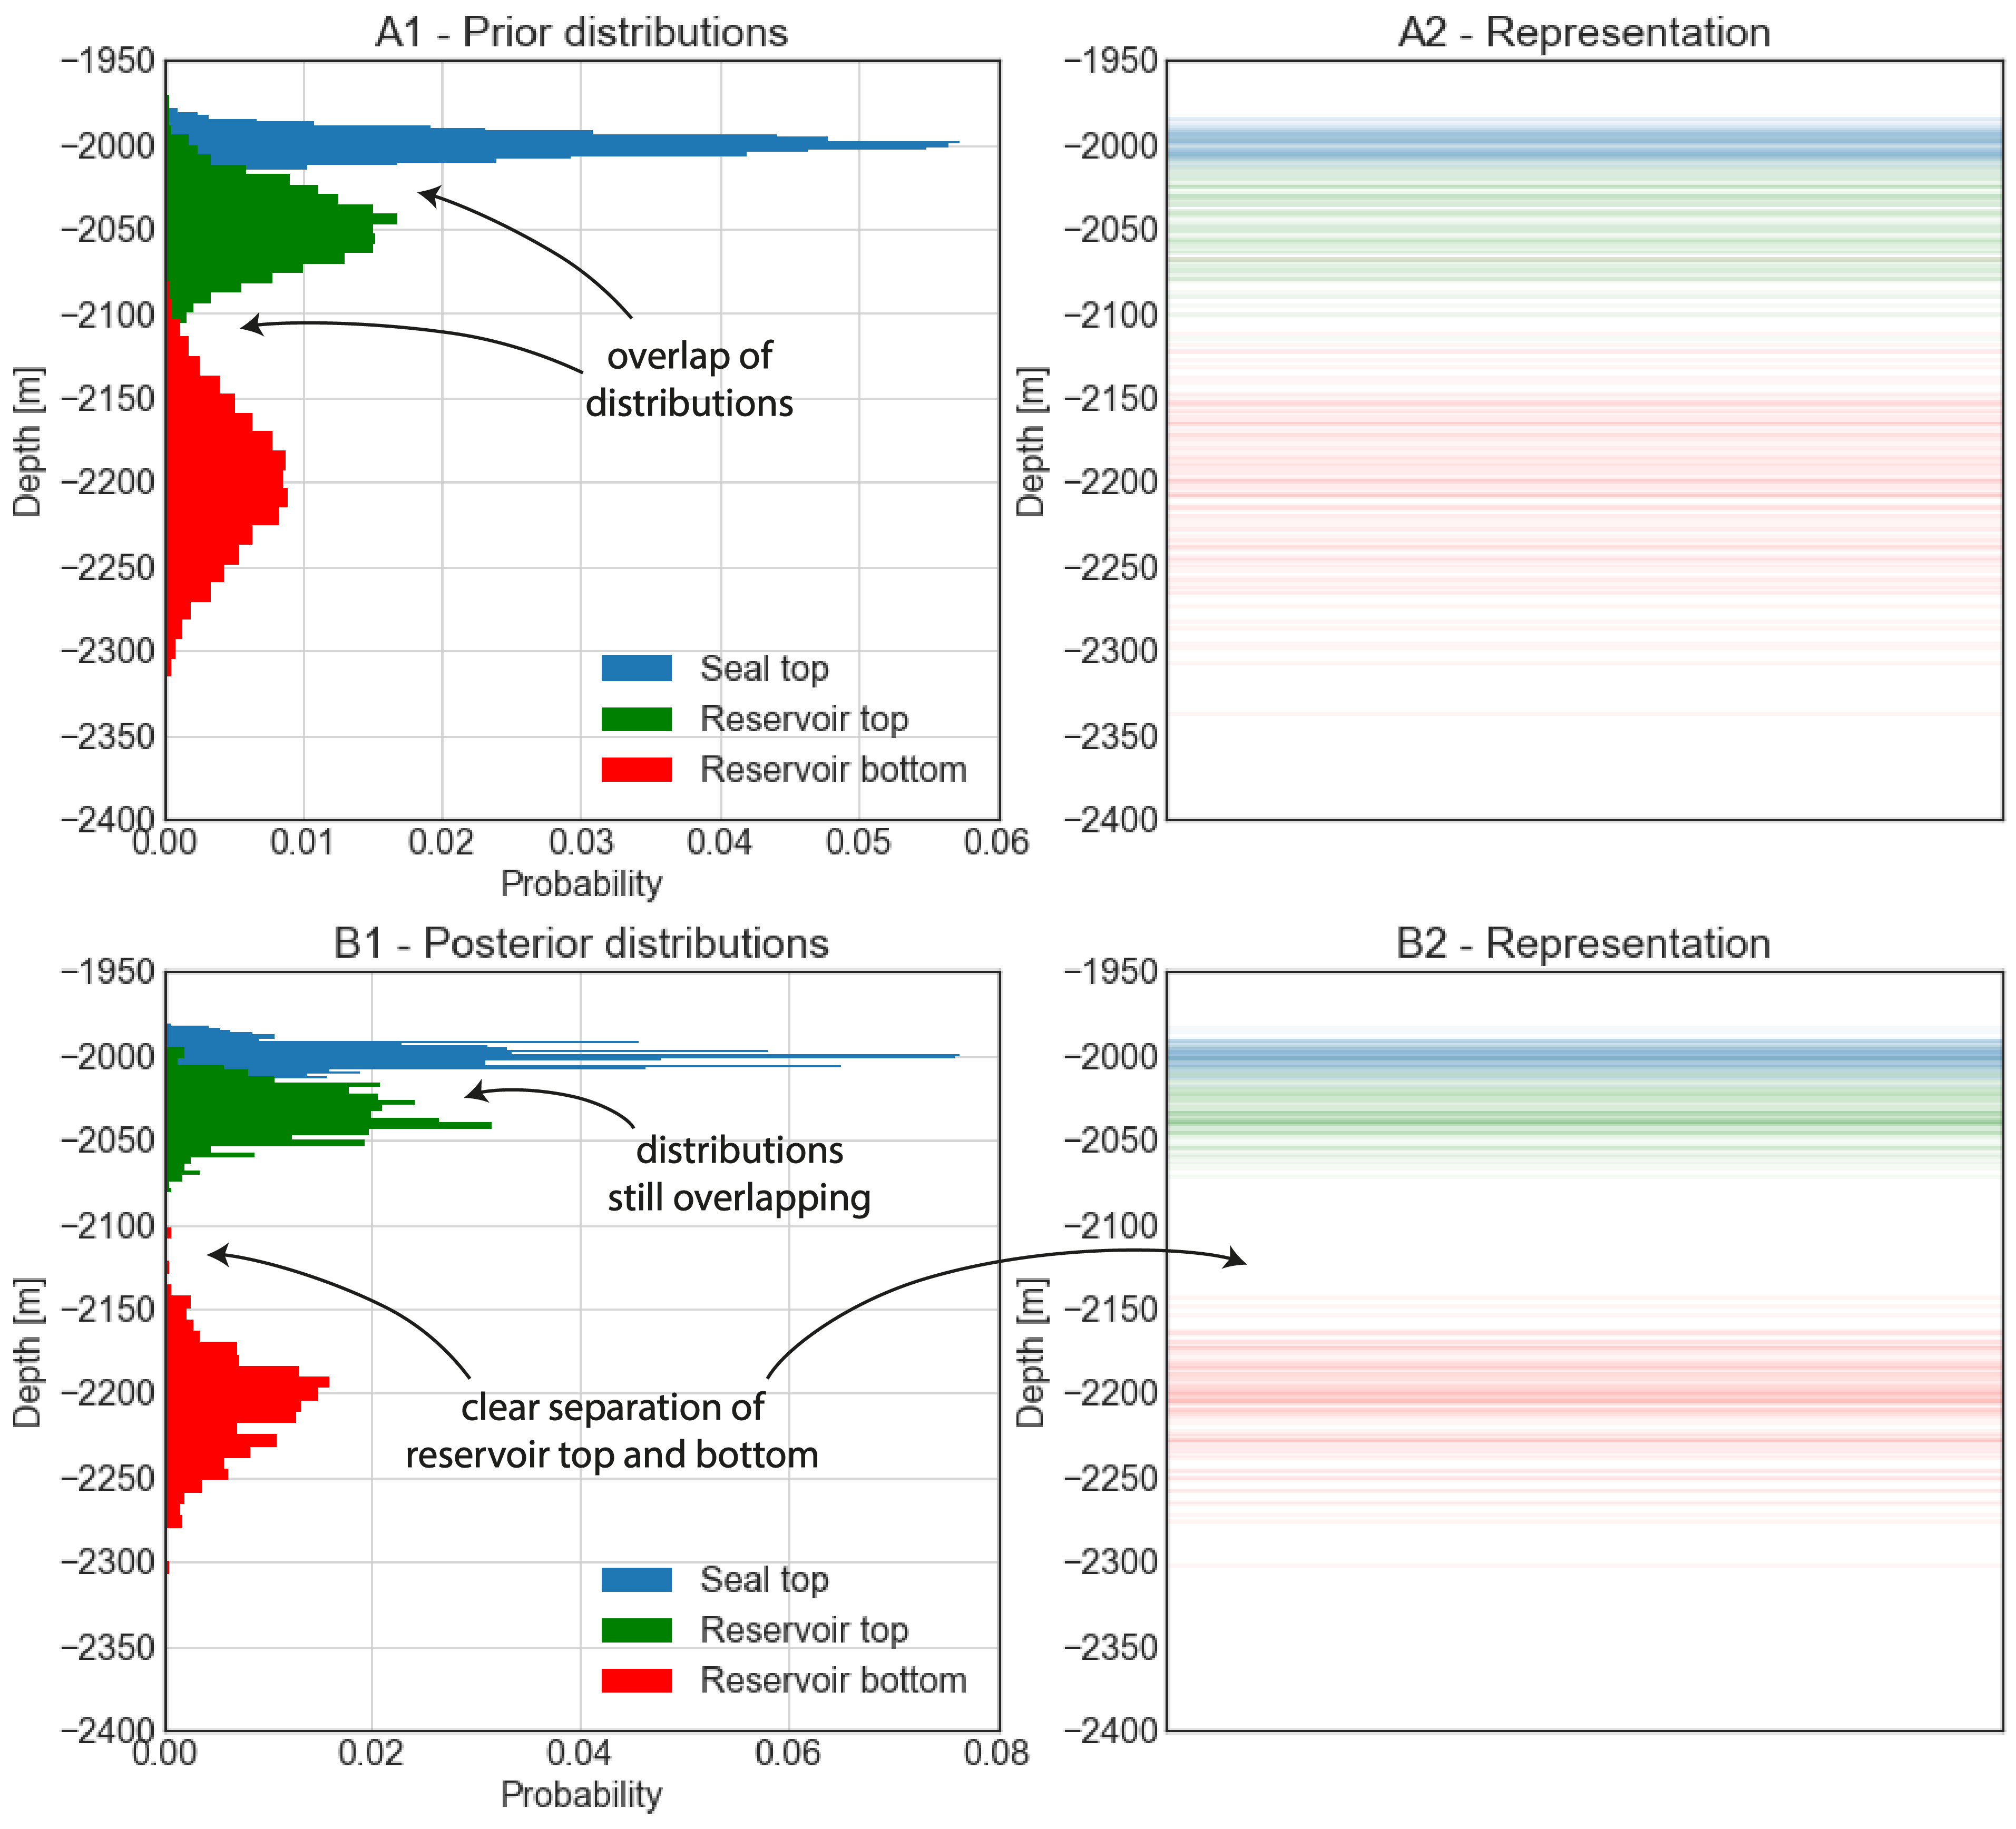
\includegraphics[width=1\textwidth]{Figures/update_moderate1.png}
				\caption{Prior (A1) and posterior distributions (A2) of the layer boundary positions in depth and respective representations (A2, B2). Bayesian inference was conducted using likelihoods defined as follows: Seal thickness: $\mu = 25~m; \sigma = 20~m$; reservoir thickness: $\mu = 180~m; \sigma = 40~m$. From (A1) to (B1), the distributions are slightly narrowed. Seal top and reservoir top distributions are still overlapping in (B1). A moderate reduction in uncertainty is also indicated by the representation in (B2), compared to (A2).}\label{fig:update_moderate1} 
			\end{figure}
			%\citet{delaVarga2016} made use of Bayesian inference to reduce the uncertainty in this type of one-dimensional model. The same was conducted here, as shown in the following.The locations of the layer boundaries are treated as priors with respective probability distributions. Now it is assumed that new observations have been made, providing additional information on the likelihoods of the thicknesses of the two layers. Likelihood functions for reservoir and seal thicknesses are introduced in the form of normal distributions, defined by means and standard deviations. These parameters vary according to nature of the observations made. Using the principle of Bayesian inference as explained in Chapter \ref{sec:bayes}, the model is updated and new posterior distributions for our true reservoir score are attained.\\
			Three representative Bayesian updating cases (10000 iterations; burn-in phase of 1000 iterations) based on different sets of likelihoods (see Table \ref{tab:1D_likelihoods}) in the 1D model are presented in the following. In each case, the layer boundaries defined in Section \ref{sec:1D_construction} were adopted as prior parameters. The various results from modeling with likelihoods, i.e. applying Bayesian inference, are compared to the original results and evaluations based on simple Monte Carlo error propagation using only priors.
			\begin{table}[h]
				\centering
			\begin{tabular}{lrrr} 
				\toprule
				(a) Inference case I - Likelihoods: layer thicknesses (normal distributions)\\  
				\midrule 
				Formation bottom & $\mu$ [m] & $\sigma$ [m]\\ 
				\midrule 
				Seal & 25 & 20 \\
				Reservoir & 180 & 40 \\
				\bottomrule
				\toprule
				(b) Inference case II - Likelihoods: layer thicknesses (normal)\\
				\midrule 
				Formation bottom & $\mu$ [m] & $\sigma$ [m]\\ 
				\midrule 
				Seal & 50 & 20 \\
				Reservoir & 180 & 40 \\
				\bottomrule
				\toprule
				(c) Inference case III - Likelihoods: layer thicknesses (normal)\\
				\midrule 
				Formation bottom & $\mu$ [m] & $\sigma$ [m]\\ 
				\midrule 
				Seal & 70 & 10 \\
				Reservoir & 100 & 30 \\
				\bottomrule
			\end{tabular}
			\caption{Thickness likelihoods defined by normal distributions, as used for the three inference cases of the 1D model.}
			\label{tab:1D_likelihoods}
			\end{table}
				
				\subsubsection{1D - Inference case I: Moderately reinforcing information}
				\begin{figure}[h]
					\begin{subfigure}{1\textwidth}
						\centering
						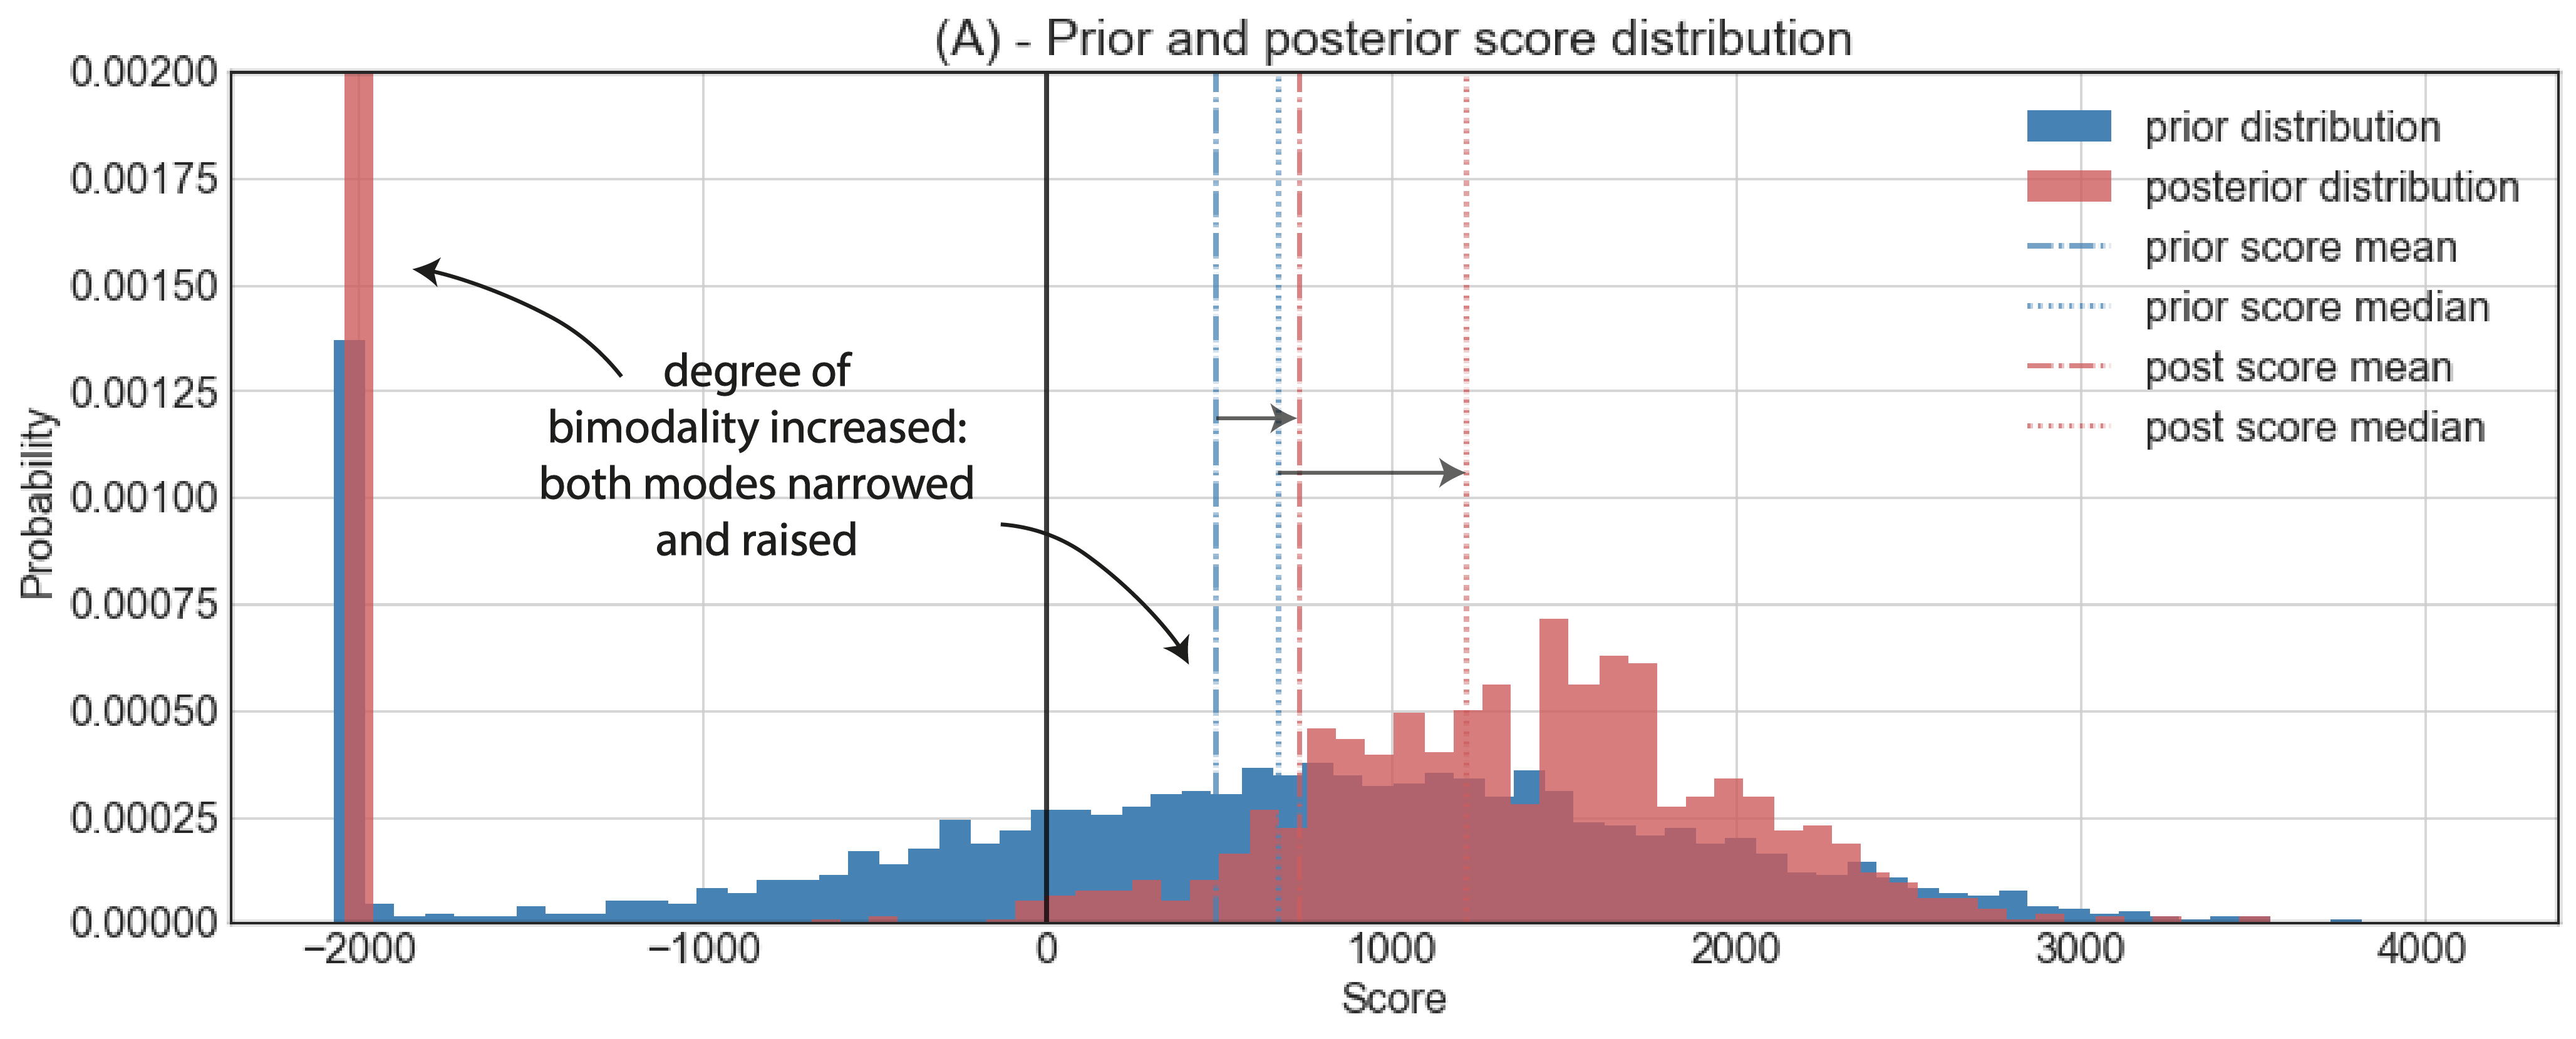
\includegraphics[width=1\linewidth]{Figures/update_moderate2.png}
						%\caption{1a}
						%\label{fig:sfig1}
					\end{subfigure}%
					\\
					\begin{subfigure}{1\textwidth}
						\centering
						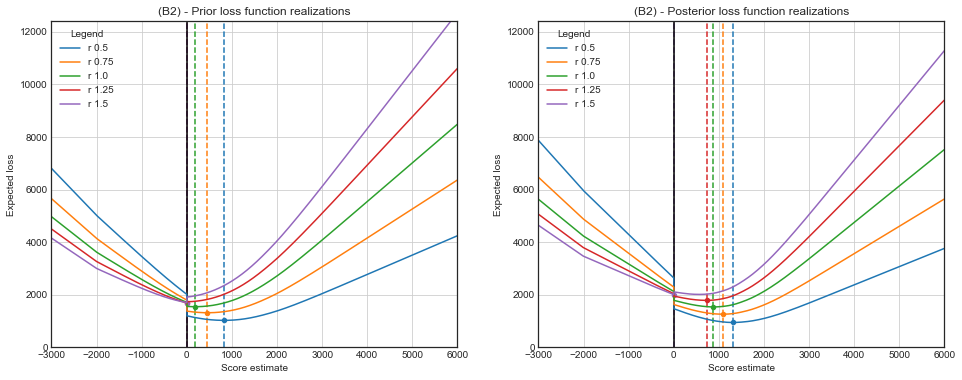
\includegraphics[width=1\linewidth]{Figures/update_moderate3.png}
						%\caption{1b}
						%\label{fig:sfig2}
					\end{subfigure}
					\caption{1D - Inference case I. Reservoir score distributions (A) and change in the realizations of expected loss for several risk parameters (B1, B2) before and after Bayesian updating based on likelihoods defined as follows: Seal thickness: $\mu = 25~m; \sigma = 20~m$; reservoir thickness: $\mu = 180~m; \sigma = 40~m$.}
					\label{fig:update_moderate2_3}
				\end{figure}				
				As can be observed in Figure \ref{fig:update_moderate1}, the uncertainty in the probability distributions for the positions of layer boundaries in depth was reduced moderately by implementing the likelihoods defined in Table \ref{tab:1D_likelihoods} (a).\\					
				Scoring was applied based on these new distributions. In Figure \ref{fig:update_moderate2_3} (A), it can be recognized that the bulk of the score distribution was shifted to the positive side of values and narrowed, approximately resembling a normal distribution there. However, the peak at -2000 was raised, while the probability of scores between -2000 and 0 was decreased to be negligible, i.e. the true score is most likely either positive or -2000, if it is negative. So while uncertainties were reduced in areas of opposite sign, the divide between these was significantly increased. The overall uncertainty seems thus to have been widely maintained and barely transformed into a problem of duality.\\
				Application of the custom loss function (Equation \ref{eq:LFR_final}) is visualized in Figure \ref{fig:update_moderate2_3}, in which the expected losses are compared before (B1) and after (B2) inference. It is observable, that by adding information about layer thickness likelihoods, Bayes actions were shifted relative to the nature of the information. In this case, the added data generally reinforced the probability of the reservoir to be sufficiently thick. Information on the seal, however, based on a normal distribution around 25~m thickness, left high uncertainty about the reliability of the seal, as the safety threshold was defined to be 20~m. Consequently, the risk of complete seal failure remained a major concern.\\				
				Increased certainty about the reservoir thickness was sufficient to shift Bayes actions to higher estimates for all actors. Estimators of the more risk-neutral actors ($r = 0.75$ to $r=1.25$) were increased the most. This has led to a slight convergence of the Bayes actions. For the risk-neutral actor, change in expected loss was negligible. For risk-friendlier actors, the expected loss was decreased, but for risk-averse actors, as they shifted from zero ("take no action") to positive estimates, increased.\\	
				%These shifts are quantified in Table \ref{tab:update_examples_all}.Expected losses are decreased for the risk-neutral and the two risk-friendlier individuals. It is clear that the expected loss was reduced the most for the risk-friendliest actor and it increased most significantly for the most risk-averse actor.
				%\begin{table}
				%	\centering
				%	\begin{tabular}[c]{| l | l | l |}
				%		\hline
				%		Risk factor \textit{r} & Shift in Bayes action & Change in expected loss \\ \hline
				%		0.50 & +~553.67 & -~105.49 \\ 
				%		0.75 & +~673.40 & -~81.67  \\ 
				%		1.00 & +~750.05 & -~33.56 \\ 
				%		1.25 & +~713.19 & +~75.71 \\ 
				%		1.50 & +~0.00 & +~282.64  \\ 
				%		\hline
				%	\end{tabular}
				%	\caption{Bla}
				%	\label{tab:update_moderate_tab}
				%\end{table}
								
				\subsubsection{1D - Inference case II: Likely reliable seal}
				\begin{figure}[h]
					\begin{subfigure}{1\textwidth}
						\centering
						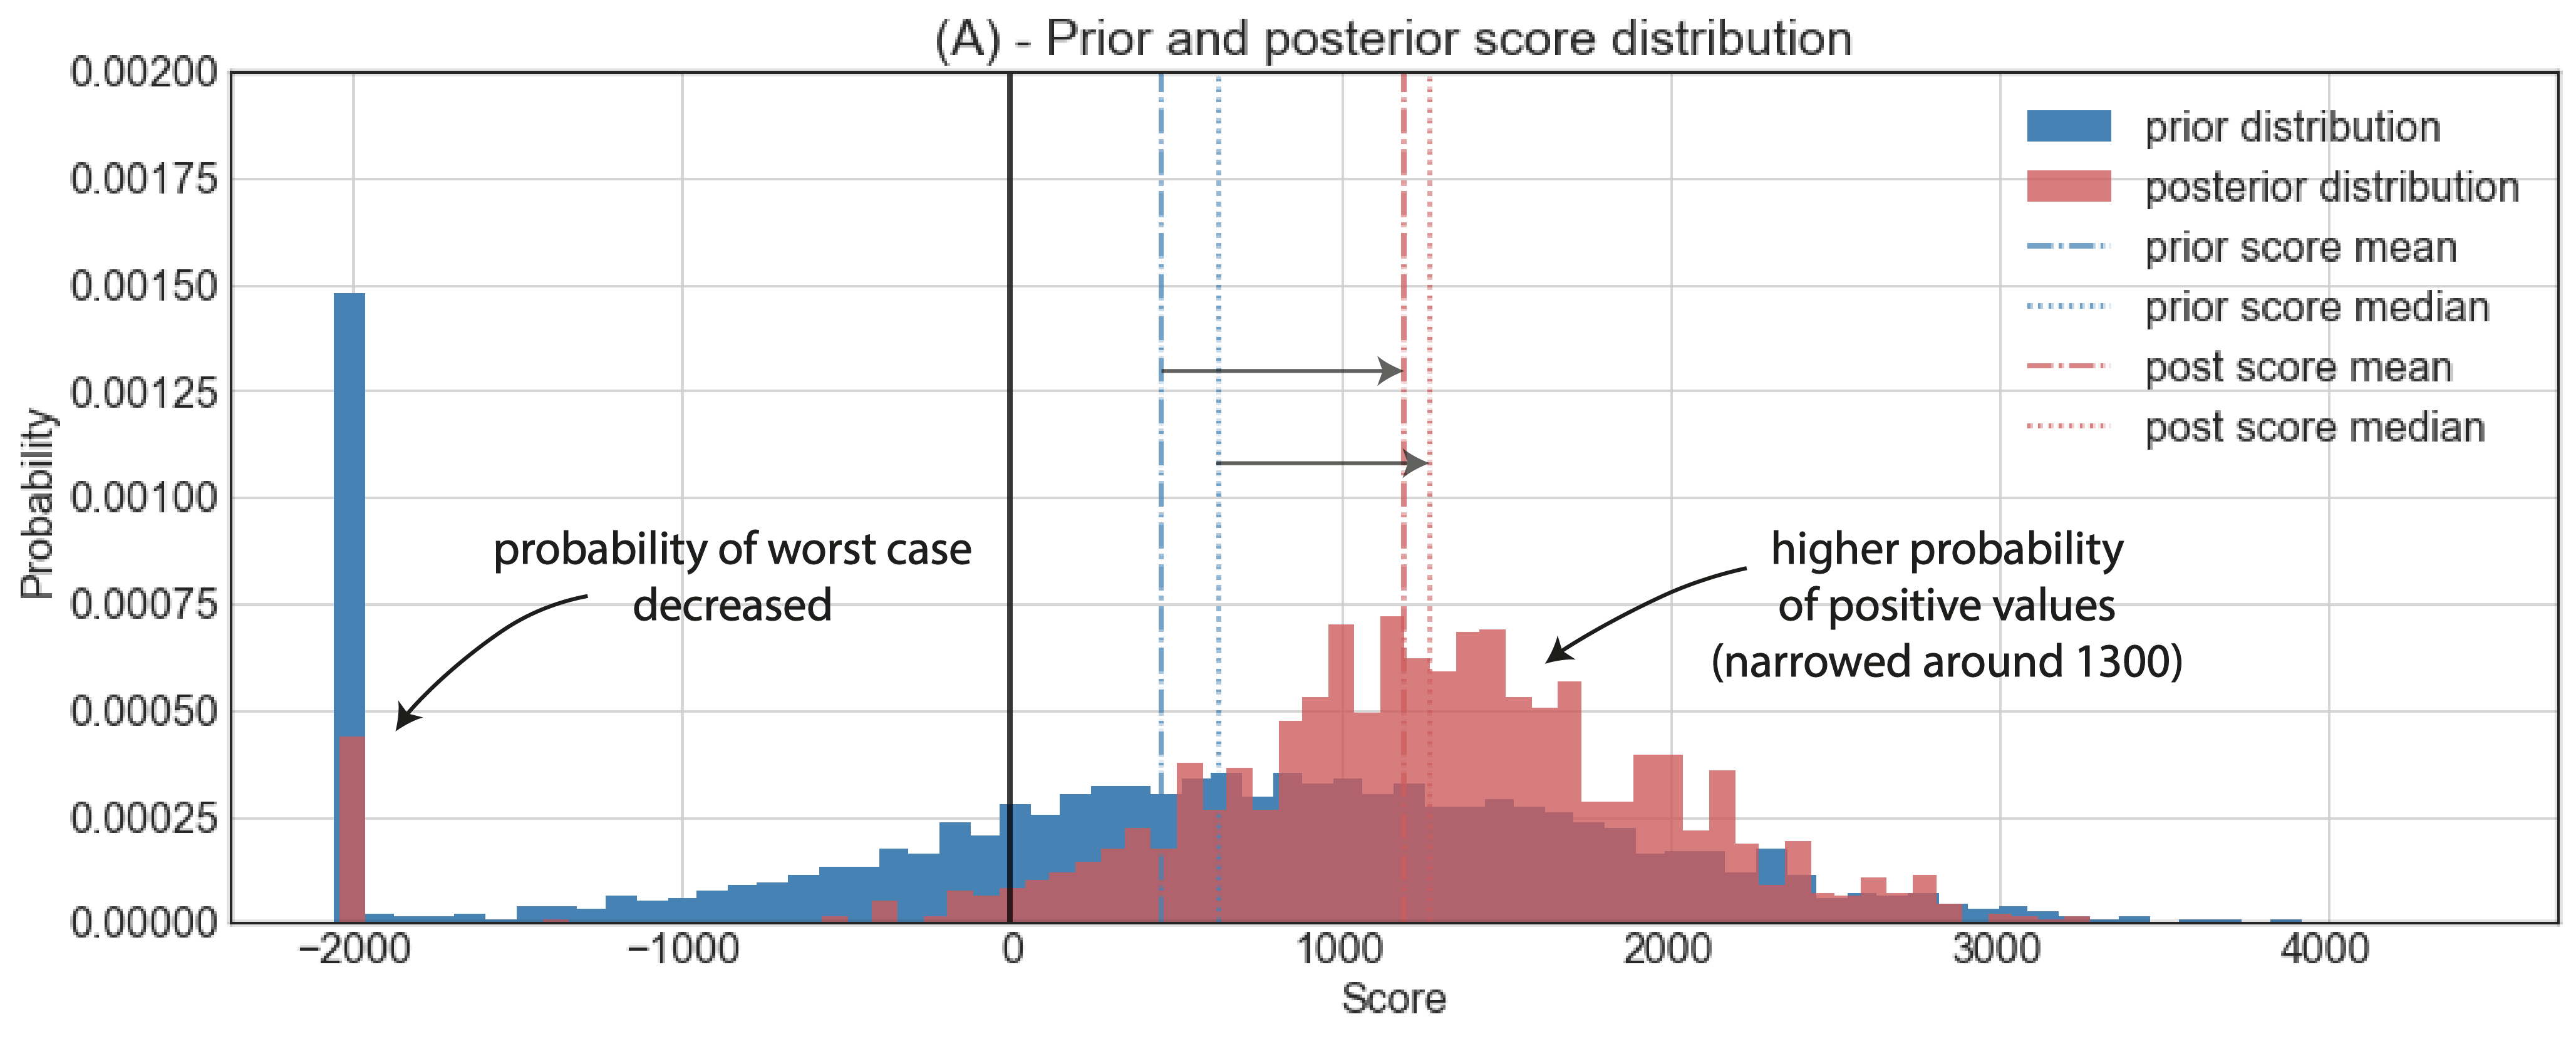
\includegraphics[width=1\linewidth]{Figures/update_goodseal2.png}
						%\caption{1a}
						%\label{fig:sfig1}
					\end{subfigure}%
					\\
					\begin{subfigure}{1\textwidth}
						\centering
						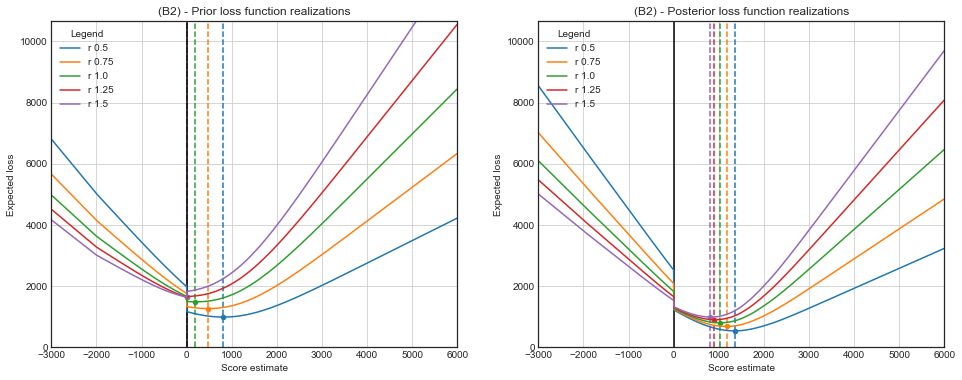
\includegraphics[width=1\linewidth]{Figures/update_goodseal3.png}
						%\caption{1b}
						%\label{fig:sfig2}
					\end{subfigure}
					\caption{1D - Inference case II. Reservoir score distributions (A) and change in the realizations of expected loss for several risk parameters (B1, B2) before and after Bayesian updating based on likelihoods defined as follows: Seal thickness: $\mu = 50~m; \sigma = 20~m$; reservoir thickness: $\mu = 180~m; \sigma = 40~m$.}
					\label{fig:update_goodseal2_3}
				\end{figure}
				In this second case, the reservoir thickness likelihood was defined in the same way as in case I (see Table \ref{tab:1D_likelihoods}). For the seal, a higher mean of 50~m chosen, favoring the likelihood of a safe thickness relative to the threshold of 20~m (see Figure \ref{fig:update_goodseal1}). Respective score results are depicted in Figure \ref{fig:update_goodseal2_3} (A). The bulk of the distribution is narrowed on the positive side of estimates. Very apparent is the significant diminishment of the "seal failure peak" at -2000. Due to this, in combination with the overall distribution narrowing, mean and median were clearly shifted to higher values and are now much closer together.\\	
				Applying the custom loss function to this new score distribution resulted in the realizations of expected loss illustrated in Figure \ref{fig:update_goodseal2_3}. Bayes actions were shifted clearly to higher estimates and expected losses of these minima were significantly reduced for all actors. The risk-neutral to risk-averse individuals seem to have profited the most, due to a large change in estimator value and decreased expected loss (Bayes risk). Compared to the foregone case, a higher degree of overall uncertainty reduction was achieved. The risk of seal failure is now much lower. Consequently, Bayes actions were not only shifted to greater values, but also narrowed significantly in their range, i.e. the optimal decisions of the different actors have converged to a much greater extent than in case I.\\		
				%This is quantified in Table \ref{tab:update_examples_all}. According to these values,  Compared to case I, the estimate shifts for both risk-friendlier actors remain approximately the same, expected losses, however, are lowered much more significantly.
				%\begin{table}
				%	\centering
				%	\begin{tabular}[c]{| l | l | l |}
				%		\hline
				%		Risk factor \textit{r} & Shift in Bayes action & Change in expected loss \\ \hline
				%		0.50 & +~522.95 & -~436.26 \\ 
				%		0.75 & +~697.73 & -~551.92  \\ 
				%		1.00 & +~855.57 & -~631.92 \\ 
				%		1.25 & +~912.43 & -~647.10 \\ 
				%		1.50 & +~819.26 & -~545.96  \\ 
				%		\hline
				%	\end{tabular}
				%	\caption{Bla}
				%	\label{tab:update_goodseal_tab}
				%\end{table}
				
				\subsubsection{1D - Inference case III: Safe seal but likely subpar reservoir thickness}
				\begin{figure}[h]
					\begin{subfigure}{1\textwidth}
						\centering
						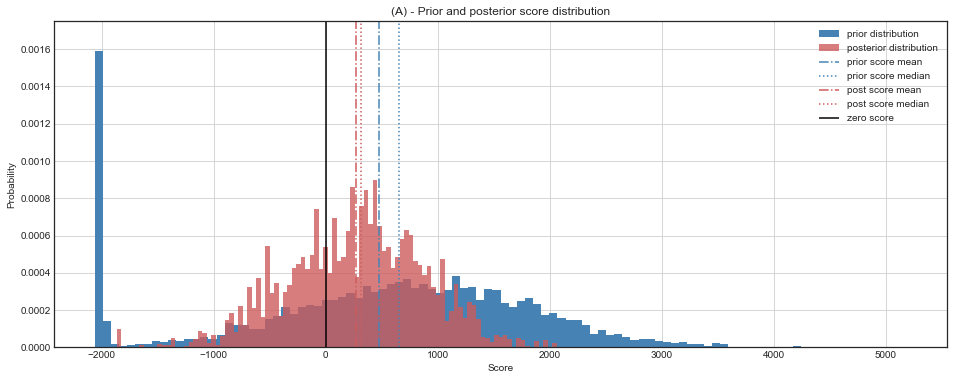
\includegraphics[width=1\linewidth]{Figures/update_smallres2.png}
						%\caption{1a}
						%\label{fig:sfig1}
					\end{subfigure}%
					\\
					\begin{subfigure}{1\textwidth}
						\centering
						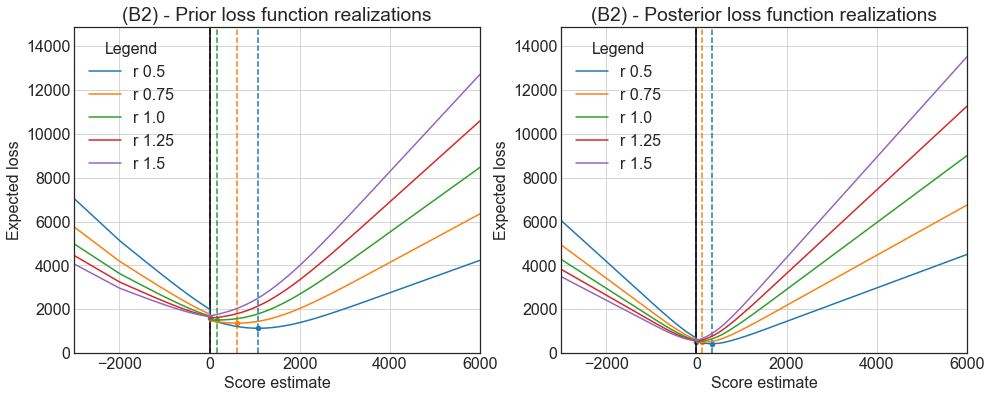
\includegraphics[width=1\linewidth]{Figures/update_smallres3.png}
						%\caption{1b}
						%\label{fig:sfig2}
					\end{subfigure}
					\caption{1D - Inference case III. Reservoir score distributions (A) and change in the realizations of expected loss for several risk parameters (B1, B2) before and after Bayesian updating based on likelihoods defined as follows: Seal thickness: $\mu = 70~m; \sigma = 10~m$; reservoir thickness: $\mu = 100~m; \sigma = 30~m$.}
					\label{fig:update_smallres2_3}
				\end{figure}
				In this third case, seal safety was ensured by using a mean of 70~m with a standard deviation of 10~m for the seal thickness likelihood. However, the new observations were assumed to provide information about the reservoir unit that makes it likely to be thinner than priorly expected (see Table \ref{tab:1D_likelihoods} (c) and Figure \ref{fig:update_smallres1})\\
				The subsequent score distribution is depicted in Figure \ref{fig:update_smallres2_3} (A). It can be seen that while the whole distribution was strongly narrowed, it also was shifted to lower and negative estimates. Mean and median are almost equal, indicating narrowing towards symmetry in the shape of a normal distribution. As seal reliability was practically guaranteed, the peak at -2000 vanished.\\				
				Based on this posterior score probability distribution, Bayes actions were shifted to lower estimates for all actors (see Figure \ref{fig:update_smallres2_3} (B2)). The risk-neutral and both risk-averse individuals find their Bayesian estimators to be zero after updating, i.e.\ bidding on a positive score is deemed to be too risky to them. There is no shift in estimate for risk-averse actors, as they already found their best estimates to be zero before updating. Notable is the large reduction of expected loss (Bayes risk) in general. The range of Bayes actions was significantly narrowed. Overall, it is apparent that uncertainty was greatly reduced (see the narrowed distribution). However, although the seal can now expected to be safe, the reservoir thickness is likely subpar. Due to this, the distribution was shifted to lower and negative values, strongly increasing the probability of an unfavorable true score. Consequently, only risk-friendly actors are willing to take action.
				%Quantified changes in the positions and values of the Bayes actions are listed in Table \ref{tab:update_examples_all}. Furthermore, the spread of expected loss values around the minima for all actors was diminished. In other words, the expected loss values of the Bayes actions are now much closer to each other.
				%\begin{table}
				%	\centering
				%	\begin{tabular}[c]{| l | l | l |}
				%		\hline
				%		Risk factor \textit{r} & Shift in Bayes action & Change in expected loss \\ \hline
				%		0.50 & -~498.98 & -~538.08 \\ 
				%		0.75 & -~346.16 & -~717.83  \\ 
				%		1.00 & -~176.13 & -~872.02 \\ 
				%		1.25 & -~0.00 & -~946.04 \\ 
				%		1.50 & -~0.00 & -~951.57  \\ 
				%		\hline
				%	\end{tabular}
				%	\caption{Bla}
				%	\label{tab:update_smallres_tab}
				%\end{table}
				% % % %
				% % % %
				%\begin{table}
				%	\centering
				%	\begin{tabular}[c]{| c || l | l || l | l || l | l |}
				%		\hline
				%		& Example I & & Example II & & Example III & \\
				%		\hline
				%		\hline
				%		\textit{r} & $\Delta$ BA & $\Delta$ EL & $\Delta$ BA & $\Delta$ EL & $\Delta$ BA & $\Delta$ EL\\ 
				%		\hline
				%		0.50 & +~553.67 & -~105.49 & +~522.95 & -~436.26 & -~498.98 & -~538.08 \\ 
				%		0.75 & +~673.40 & -~81.67 & +~697.73 & -~551.92 & -~346.16 & -~717.83  \\ 
				%		1.00 & +~750.05 & -~33.56 & +~855.57 & -~631.92 & -~176.13 & -~872.02 \\ 
				%		1.25 & +~713.19 & +~75.71 & +~912.43 & -~647.10 & -~0.00 & -~946.04 \\ 
				%		1.50 & +~0.00 & +~282.64 & +~819.26 & -~545.96 & -~0.00 & -~951.57  \\ 
				%		\hline
				%	\end{tabular}
				%	\caption{Changes in Bayes action (BA) and minimal expected loss (EL) for Bayesian updating cases I, II and III and respective actors with risk parameters $r$.}
				%	\label{tab:update_examples_all}
				%\end{table}
				% % % %
				% % % %
				%\begin{table}
				%		\begin{tabular}[c]{| l | l | l |}
				%			\hline
				%			Risk factor \textit{r} & Shift in Bayes action & Change in expected loss \\ \hline
				%			0.50 & -~498.98 & -~538.08 \\ 
				%			0.75 & -~346.16 & -~717.83  \\ 
				%			1.00 & -~176.13 & -~872.02 \\ 
				%			1.25 & -~0.00 & -~946.04 \\ 
				%			1.50 & -~0.00 & -~951.57  \\ 
				%			\hline
				%		\end{tabular}
				%		\caption{Bla}
				%		\label{tab:update_examples_all}
				%\end{table}
			%\subsection{General 1D model inference results}
			%This conceptual application in an abstract 1D geological model already serves to illuminate some of the main effects of Bayesian inference on decision-making. Three main mechanisms were observable in these cases: 
			%\begin{enumerate}
			%	\item \textbf{Lateral shifting} of the score distribution and consequent shift in Bayes actions along the axis of possible score estimates, while their expected losses remain approximately constant. To a certain degree, this seems to be independent from the overall uncertainty reduction and is primarily related to the shift of probability to a different area. According to this observation, uncertainty reduction is not a necessary condition to significantly alter the decisions for all individuals. 
				%An incentive to bid on higher estimates is given solely by the shift of the posterior distribution to higher values, while the inherited degree of uncertainty may remain the same.
			%	\item \textbf{Narrowing} of the score probability distribution, due to uncertainty reduction and consequent convergence of the Bayes actions of different actor's towards a similar estimate. Additionally, expected loss seem to decrease with uncertainty. If perfect information about our parameters was available, all individuals would bid on the same estimate and expected a loss of zero. 
			%	\item \textbf{Dualization} of uncertainty, apparently due to reduction of uncertainty that narrows probability to areas of two possible outcomes, such as success and failure. The area at which uncertainty is reduced seems to be of significance. A high reduction of uncertainty in the form of standard deviation near a cut-off threshold value seems to lead to a transformation of the nature of uncertainty to a problem of duality. CONNECTION TO SHIFTING???
			%\end{enumerate}
			%The second mechanism, i.e. uncertainty reduction, can thus presumed to be most significant regarding the process of "good" decision-making, as actor's wish to minimize their expected loss from bidding on an estimate. In an optimal case, this would come in combination with a shift of probabilities (first mechanism) to more positive values, so that a higher economic value may be returned from the acquisition of information.
			%As can be expected intuitively, reassurance of positive scores, for example by narrowing of the distribution of scores on the side of positive estimates or by reducing the occurrence of negative extrema, leads to shifts towards higher Bayes action estimates for all actors. Conversely, actors are discouraged to expect gains when facing a higher probability of negative scores. Unsurprising is also the inverse behavior of risk-averse and risk-friendly individuals. However, it is most notable that a reduction of uncertainty in any case leads to a diminished spread of Bayes actions between all actors. In other words, given better information about the true value of the reservoir, different actors come to more similar decisions. Given perfect information, all actors would presumably choose the same estimate, which would equal the true score.	
			
		\section{3D geological reservoir model results}
		In the following, we present the results from applying the methods to the synthetic 3D structural geological model. Several representative examples of posterior models based on the use of different likelihoods are referenced to the original prior model. For each simulation, 1,000 sampling steps were conducted, with a burn-in phase of 50 iterations for MCMC sampling. However, for computational reasons, Shannon entropy visualization was based on 200 sampling steps and a burn-in phase of 50 iterations. We consider in particular the following measures for the comparison of results: (1) Shannon entropy, (2) occurrence of trap control mechanisms, (3) resulting recoverable oil volumes and (4) consequent realization of expected losses and related Bayes actions (i.e. decisions).
		
		\subsection{3D - Prior model}\label{sec:prior_model3D}
		To generate a set of reference results, a prior model was first generated by running a simple simulation of Monte Carlo sampling considering only the uncertainty of prior parameters. No likelihood functions were included. The prior parameter uncertainties, defined in Table \ref{tab:3D_prior_parameters} were chosen to be identical for all posterior simulations.
		\begin{table}[h]
		\centering
		\begin{tabular}{lrrr} 
			\toprule
			(a) Uncertainty: layer boundaries $z$-position (normal distributions)\\  
			\midrule 
			Formation bottom & $\mu$ [m] & $\sigma$ [m]\\ 
			\midrule 
			Overlying & 0 & 40 \\
			Sandstone 2 & 0 & 60 \\
			Shale (Seal) & 0 & 80\\ 
			Sandstone 1 (Reservoir) & 0 & 100 \\
			\bottomrule
			\toprule
			(b) Uncertainty: normal fault offset (skew normal distribution)\\
			\midrule
			Fault side & $\mu$ [m] & $\sigma$ [m] & $\alpha$\\
			\midrule
			Hanging wall offset & 0 & -~150 & -~2\\
			\bottomrule 
		\end{tabular}
		\caption{Prior parameter uncertainties defined by distributions with respective means $\mu$, standard deviations $\sigma$ and shape factor $\alpha$, as used in all model simulations. Points belonging to the same layer interface share the same normal distribution (a). The offset uncertainty (b) is based on a skew normal distribution that affects all positional points in the hanging wall.}
		\label{tab:3D_prior_parameters}
		\end{table}
		\begin{figure}[h]
			\centering
			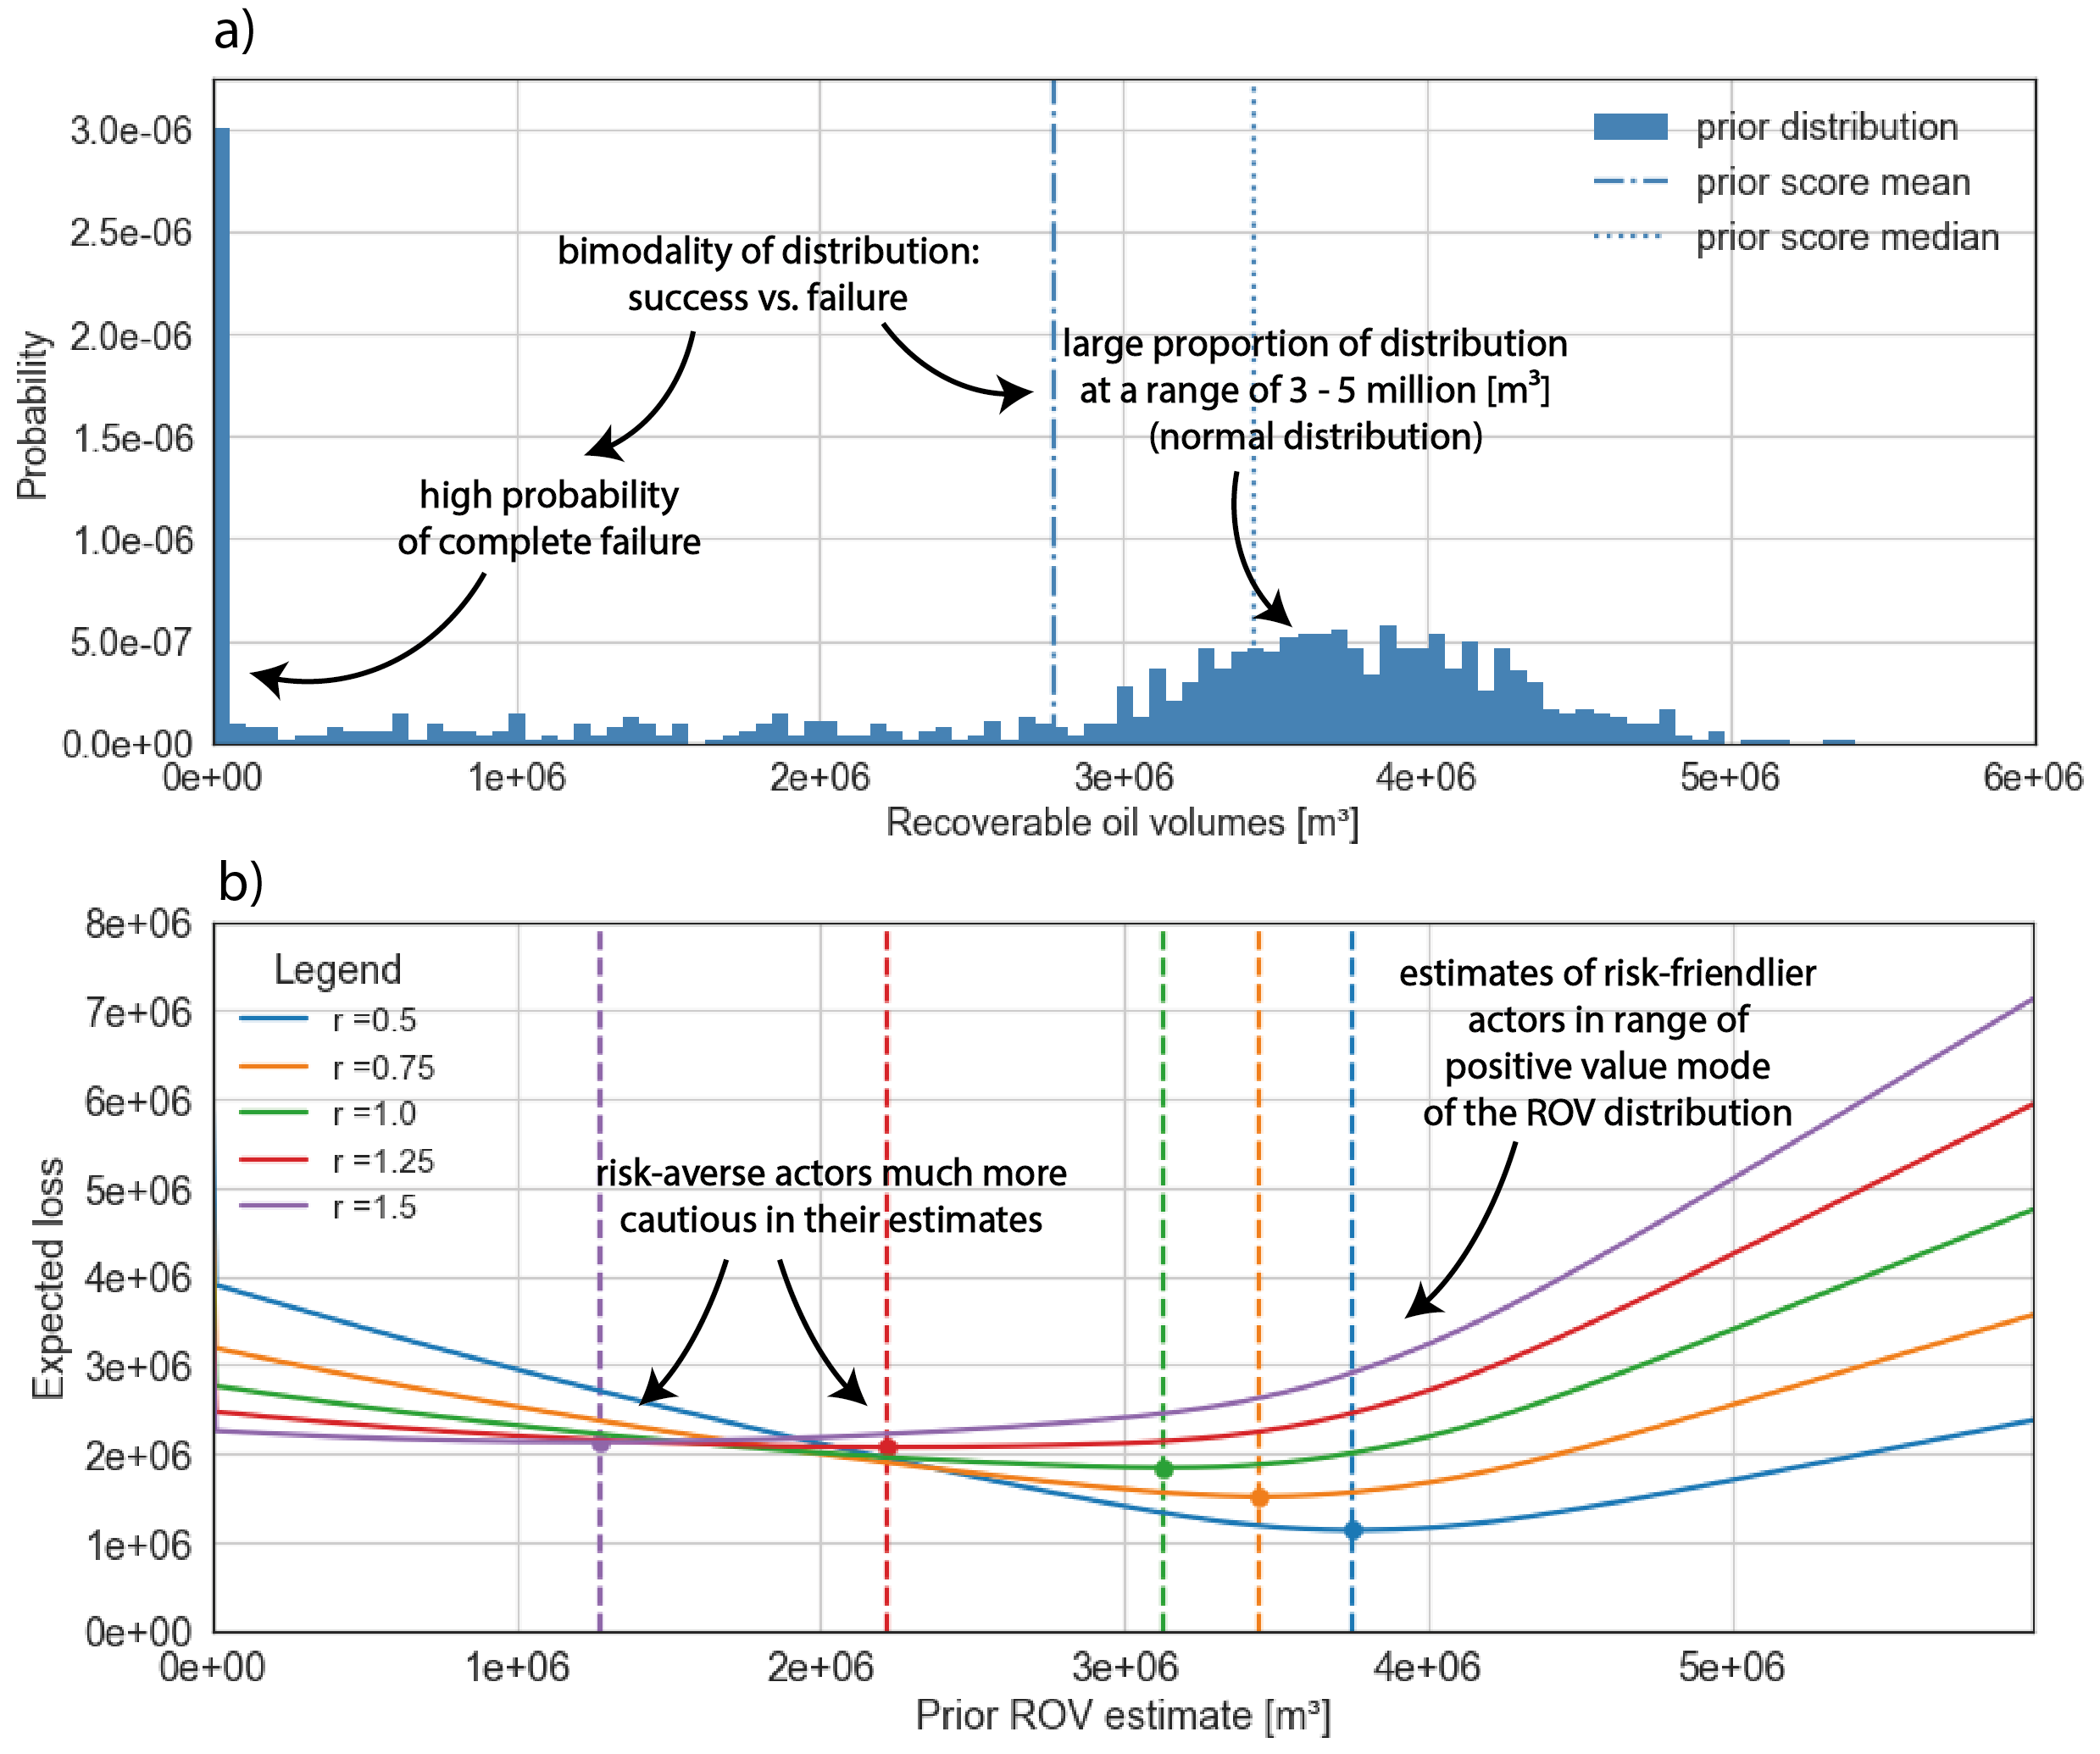
\includegraphics[width=1\textwidth]{Figures/M_prior}
			\caption{Recoverable oil volumes probability distribution for the prior 3D model (a) and respective realization of the custom loss function (b).}\label{fig:M_prior}
		\end{figure}\\
		The nature of the prior uncertainties was visualized using Shannon entropy (see Figure \ref{fig:ML1} (a)). High entropies can be seen at and near the possible locations of layer boundaries. This effect was strongly amplified by the offset uncertainty in the footwall, where the highest entropies are found.\\
		The occurrence of the different mechanisms of maximum trap control were traced for all simulations and labeled as follows:
		\begin{enumerate}
		\item \textbf{SPILL POINT:} Migration related to the anticlinal spill point of the trap.
		\item \textbf{LEAK UNDER:} Leakage due to juxtaposition of the reservoir with formations underlying the seal in the hanging wall.
		\item \textbf{LEAK OVER:} Leakage due to juxtaposition of the reservoir with formations overlying the seal in the hanging wall. This was defined to lead to full leakage and complete failure of the trap.
		\item \textbf{STRAT:} Leakage due to stratigraphical connections of the trap to seal-overlying units, i.e. stratigraphical breaches of the seal. Full leakage and trap failure were assumed for this mechanism as well.
		\item \textbf{UNCLEAR:} Label defined to track cases in which a mechanism was not recognized. This is deemed an indicator for failures of the algorithms or the computation, i.e. the reliability of the overall model and incorporated functions. 
		\end{enumerate}
		It is shown in Figure \ref{fig:ML1} (c) that all four relevant mechanisms occurred for the prior model. The dominant factor is the anticlinal spill point accounting for more than 60\% of model realizations. It is followed by cross-fault leakage labeled "LEAK UNDER" ($\sim20\%$) and "LEAK OVER" ($\sim13\%$). Stratigraphical breaches of the seal were registered to be decisive in only about 3\% of iterations. A satisfactory reliability of model algorithms and computation is indicated by the lack of unrecognized mechanisms.\\
		Recoverable oil volumes were calculated for each model iteration and plotted as a probability distribution in Figure \ref{fig:M_prior} (a). It can clearly be seen that while a large portion of the distribution is found in a range of highly positive volumes, forming a normal distribution shape around 3.8 million m$^3$, there is also a high probability of complete failure, i.e. for the trap volume to be zero. This results in a bimodal characterization with low probability of the ROV to be found between zero and 3 million m$^3$.\\
		Consequently, applying the custom loss function to this distribution resulted in divergent Bayes actions for the different risk-affine actors (see Figure \ref{fig:M_prior} (b)). Although all actors find their estimators to be positive, only the risk-neutral to risk-friendliest actors come close to the described positive mode of the distribution (ROV $> 3*10^6$ m$^3$). Risk-averse individuals bid on significantly lower estimates. It can also be observed that expected losses resulted to be generally lower for risk-affine actors. It can be presumed that the divergence of different Bayes actions was caused by the bimodality of the ROV probability distribution.
		
		\subsection{3D - Posterior model I: Seal and reservoir likely thick}
		\begin{table}[h]
			\centering
			\begin{tabular}{lrr} 
				\toprule
				Model I - Likelihoods: layer thicknesses (normal distributions)\\  
				\midrule 
				Formation & $\mu$ [m] & $\sigma$ [m]\\ 
				\midrule 
				Sandstone 2 & 150 & 30 \\
				Shale (Seal) & 350 & 30\\ 
				Sandstone 1 (Reservoir) & 250 & 30 \\
				\bottomrule
			\end{tabular}
			\caption{Layer thickness likelihoods determined by normal distributions as used for posterior model I.}
			\label{tab:ML1_likelihoods}
		\end{table}
		\begin{figure}[p!]
			\centering
			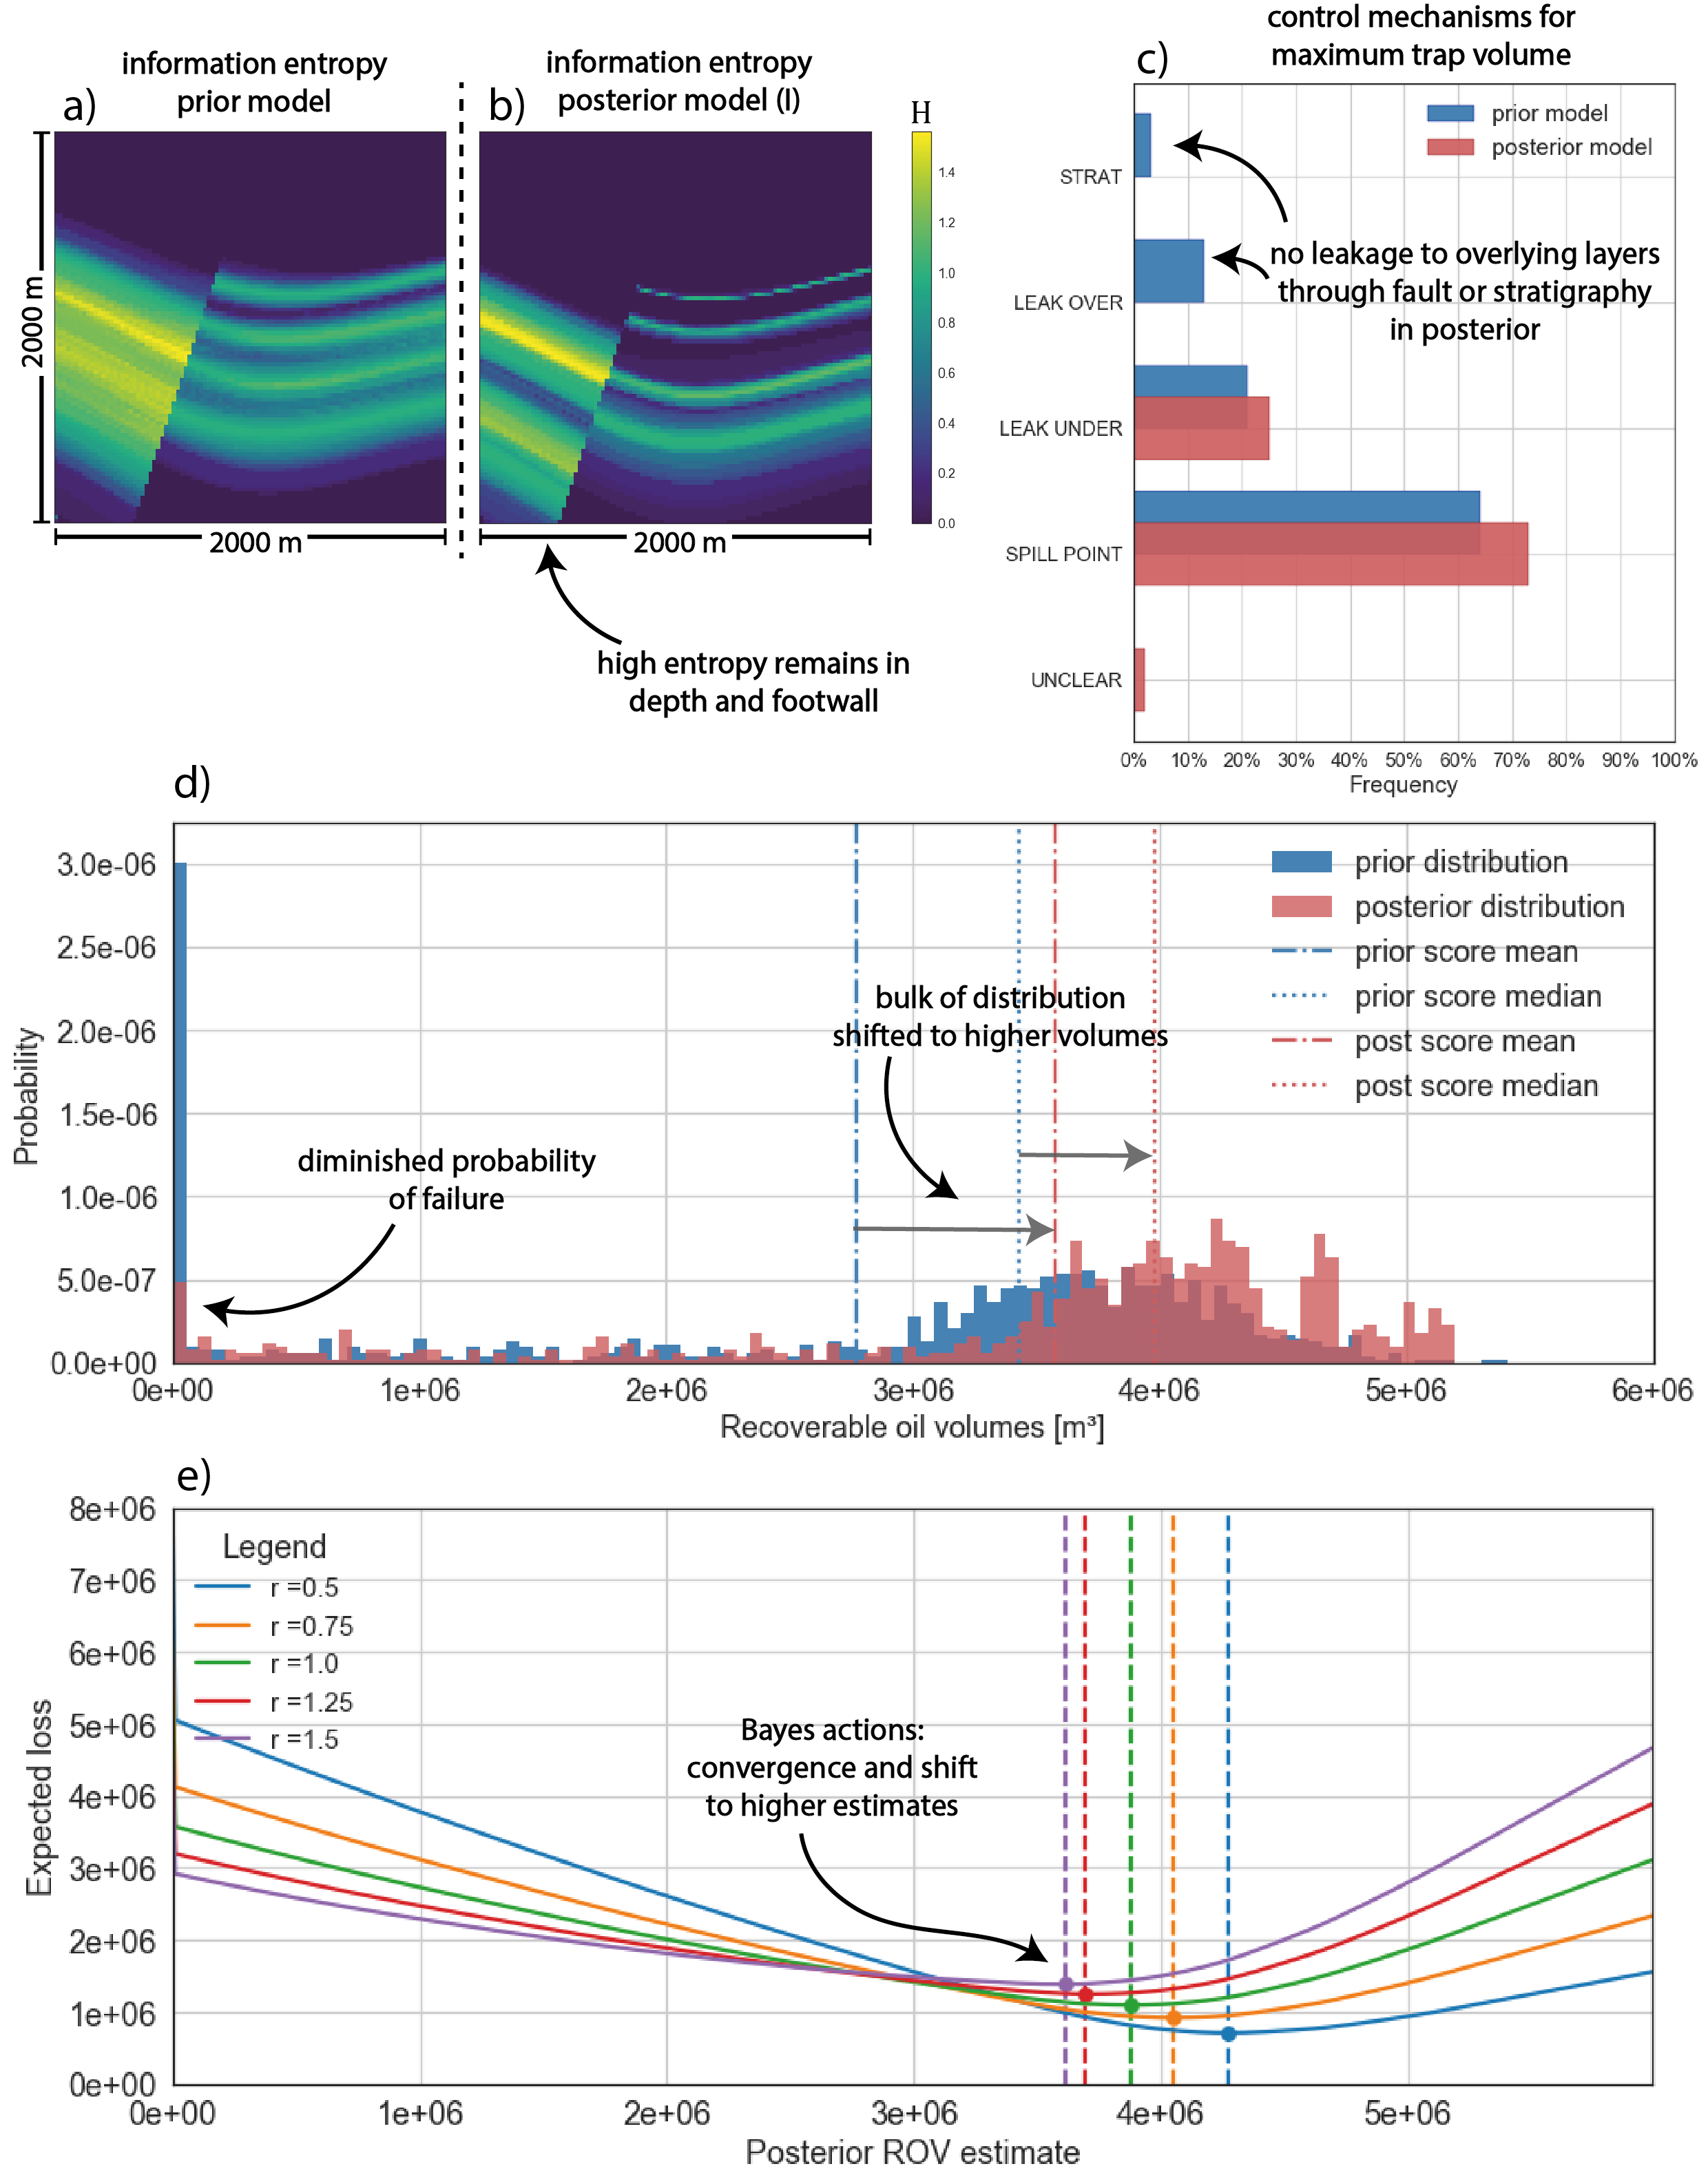
\includegraphics[width=1\textwidth]{Figures/ML1}
			\caption{Summary of results from evaluating posterior model I (3D). Shannon entropies in prior (a) and posterior (b) are compared. So are the mechanisms of maximum trap volume control (c). Prior and posterior ROV probability distributions are shown in (d). Respective loss function and Bayes actions are plotted in (e).}\label{fig:ML1}
		\end{figure}		
		For the simulation of this first posterior model, thickness likelihoods for the three central layers were included in the probabilistic model. These were defined in a way that reinforced the probabilities of the relevant layers to be significantly thick (see Table \ref{tab:ML1_likelihoods}). Respective results are summarized in Figure \ref{fig:ML1}.\\
		Considering the changes in Shannon entropy, it can be seen that the uncertainty about layer interface positions in $z$ was clearly reduced in the footwall. Information entropy was also decreased in the middle section of the hanging wall, but remained high in upper and lower parts, presumably due to the remaining influence of the offset uncertainty.\\
		Regarding trap volume control (Figure \ref{fig:ML1} (c)), only spill point-related migration ("SPILL POINT") and cross-fault leakage due to juxtaposition with permeable layers below the seal in the hanging wall ("LEAK UNDER") remained relevant in the posterior model. As no occurrences of leakage through overlying layers were observed, these two main mechanisms increased in frequency, while staying proportionally the same to one another. It can be presumed, that by introducing the respective likelihoods, a high thickness of the seal was ensured, as can also be recognized in Figure \ref{fig:ML1} (b). This not only made stratigraphic leakage in this model impossible, but also enforced a favorable SSF. A minor emergence of unrecognized control factors ("UNCLEAR") suggests that, for a few iterations, the model was possibly not correctly computable or the structural analysis failed for a different reason.\\
		The bulk that accounted for the positive mode in the prior ROV distribution was raised and shifted laterally to higher values, while the probability of failure (ROV = 0) was diminished significantly (see Figure Figure \ref{fig:ML1} (d)). This can presumably be explained by the disappearance of leakage to overlying formations as a trap control mechanism, which was programmed to always lead to complete failure of the trap volume.\\
		As the probability of failure and thus the bimodality of the probability distribution were diminished, all Bayes actions were shifted to higher estimates, most significantly those of the two risk-averse individuals (see Figure \ref{fig:ML1} (e)). These have thus converged into an area of similar expectations. Additionally, expected losses (Bayes risks) were lowered overall. The posterior state of knowledge, provided by the updated model, encouraged even the most risk-averse decision-maker to expect recoverable oil volumes from 3.5 million m$^3$ upwards.
		
		\subsection{3D - Posterior model II: Likely thin reservoir formation}%ML3
		\begin{table}[h]
			\centering
			\begin{tabular}{lrr} 
				\toprule
				Model II - Likelihoods: layer thicknesses (normal distributions)\\  
				\midrule 
				Formation & $\mu$ [m] & $\sigma$ [m]\\ 
				\midrule 
				Sandstone 2 & 300 & 30 \\
				Shale (Seal) & 400 & 40\\ 
				Sandstone 1 (Reservoir) & 50 & 10 \\
				\bottomrule
			\end{tabular}
			\caption{Layer thickness likelihoods determined by normal distributions as used for posterior model II.}
			\label{tab:ML3_likelihoods}
		\end{table}
		For the second model, thickness likelihoods were defined in a way that reinforced the probability of a very thick seal, but at the same time restricted the reservoir formation to a likely significantly thinner thickness of around 50 m (see Table \ref{tab:ML3_likelihoods}). The results (see Figure \ref{fig:ML3}) are very similar, in fact almost identical, to those of model I above. This can be explained by the influence of leak and spill point. As the shape of the general structure itself was not defined to be uncertain, the position of the anticlinal spill point relative to the fault top remains mostly unchanged, irrespective of layer thickness variations. Thus, reservoir thickness is only a secondary factor to trap volume control. Assuming fixed values for all other parameters, the maximum fill horizon is most likely the same for a 300 m as for a 50 m thick reservoir unit. The thickness of the reservoir only becomes significant, if it is thin enough to locate the respective layer bottom above the leak and spill point depth in the trap section. Ultimately, the spill point appears to be the primariy limiting factor to maximum trap fill. It can furthermore be derived from this that the maximum trap volume potential, as defined by the given structural features, is already represented in the ROV probability distribution of the prior model. After examining Figure \ref{fig:ML1} (d), it seems that this overall maximum volume is found at approximately 5.7 millon m$^3$. Higher values were not observed in any other model realization and are presumed to be unattainable due to the restriction given by the spill point.
	
		\subsection{3D - Posterior model III: Likely thin seal}%ML2
		\begin{figure}[p!]
			\centering
			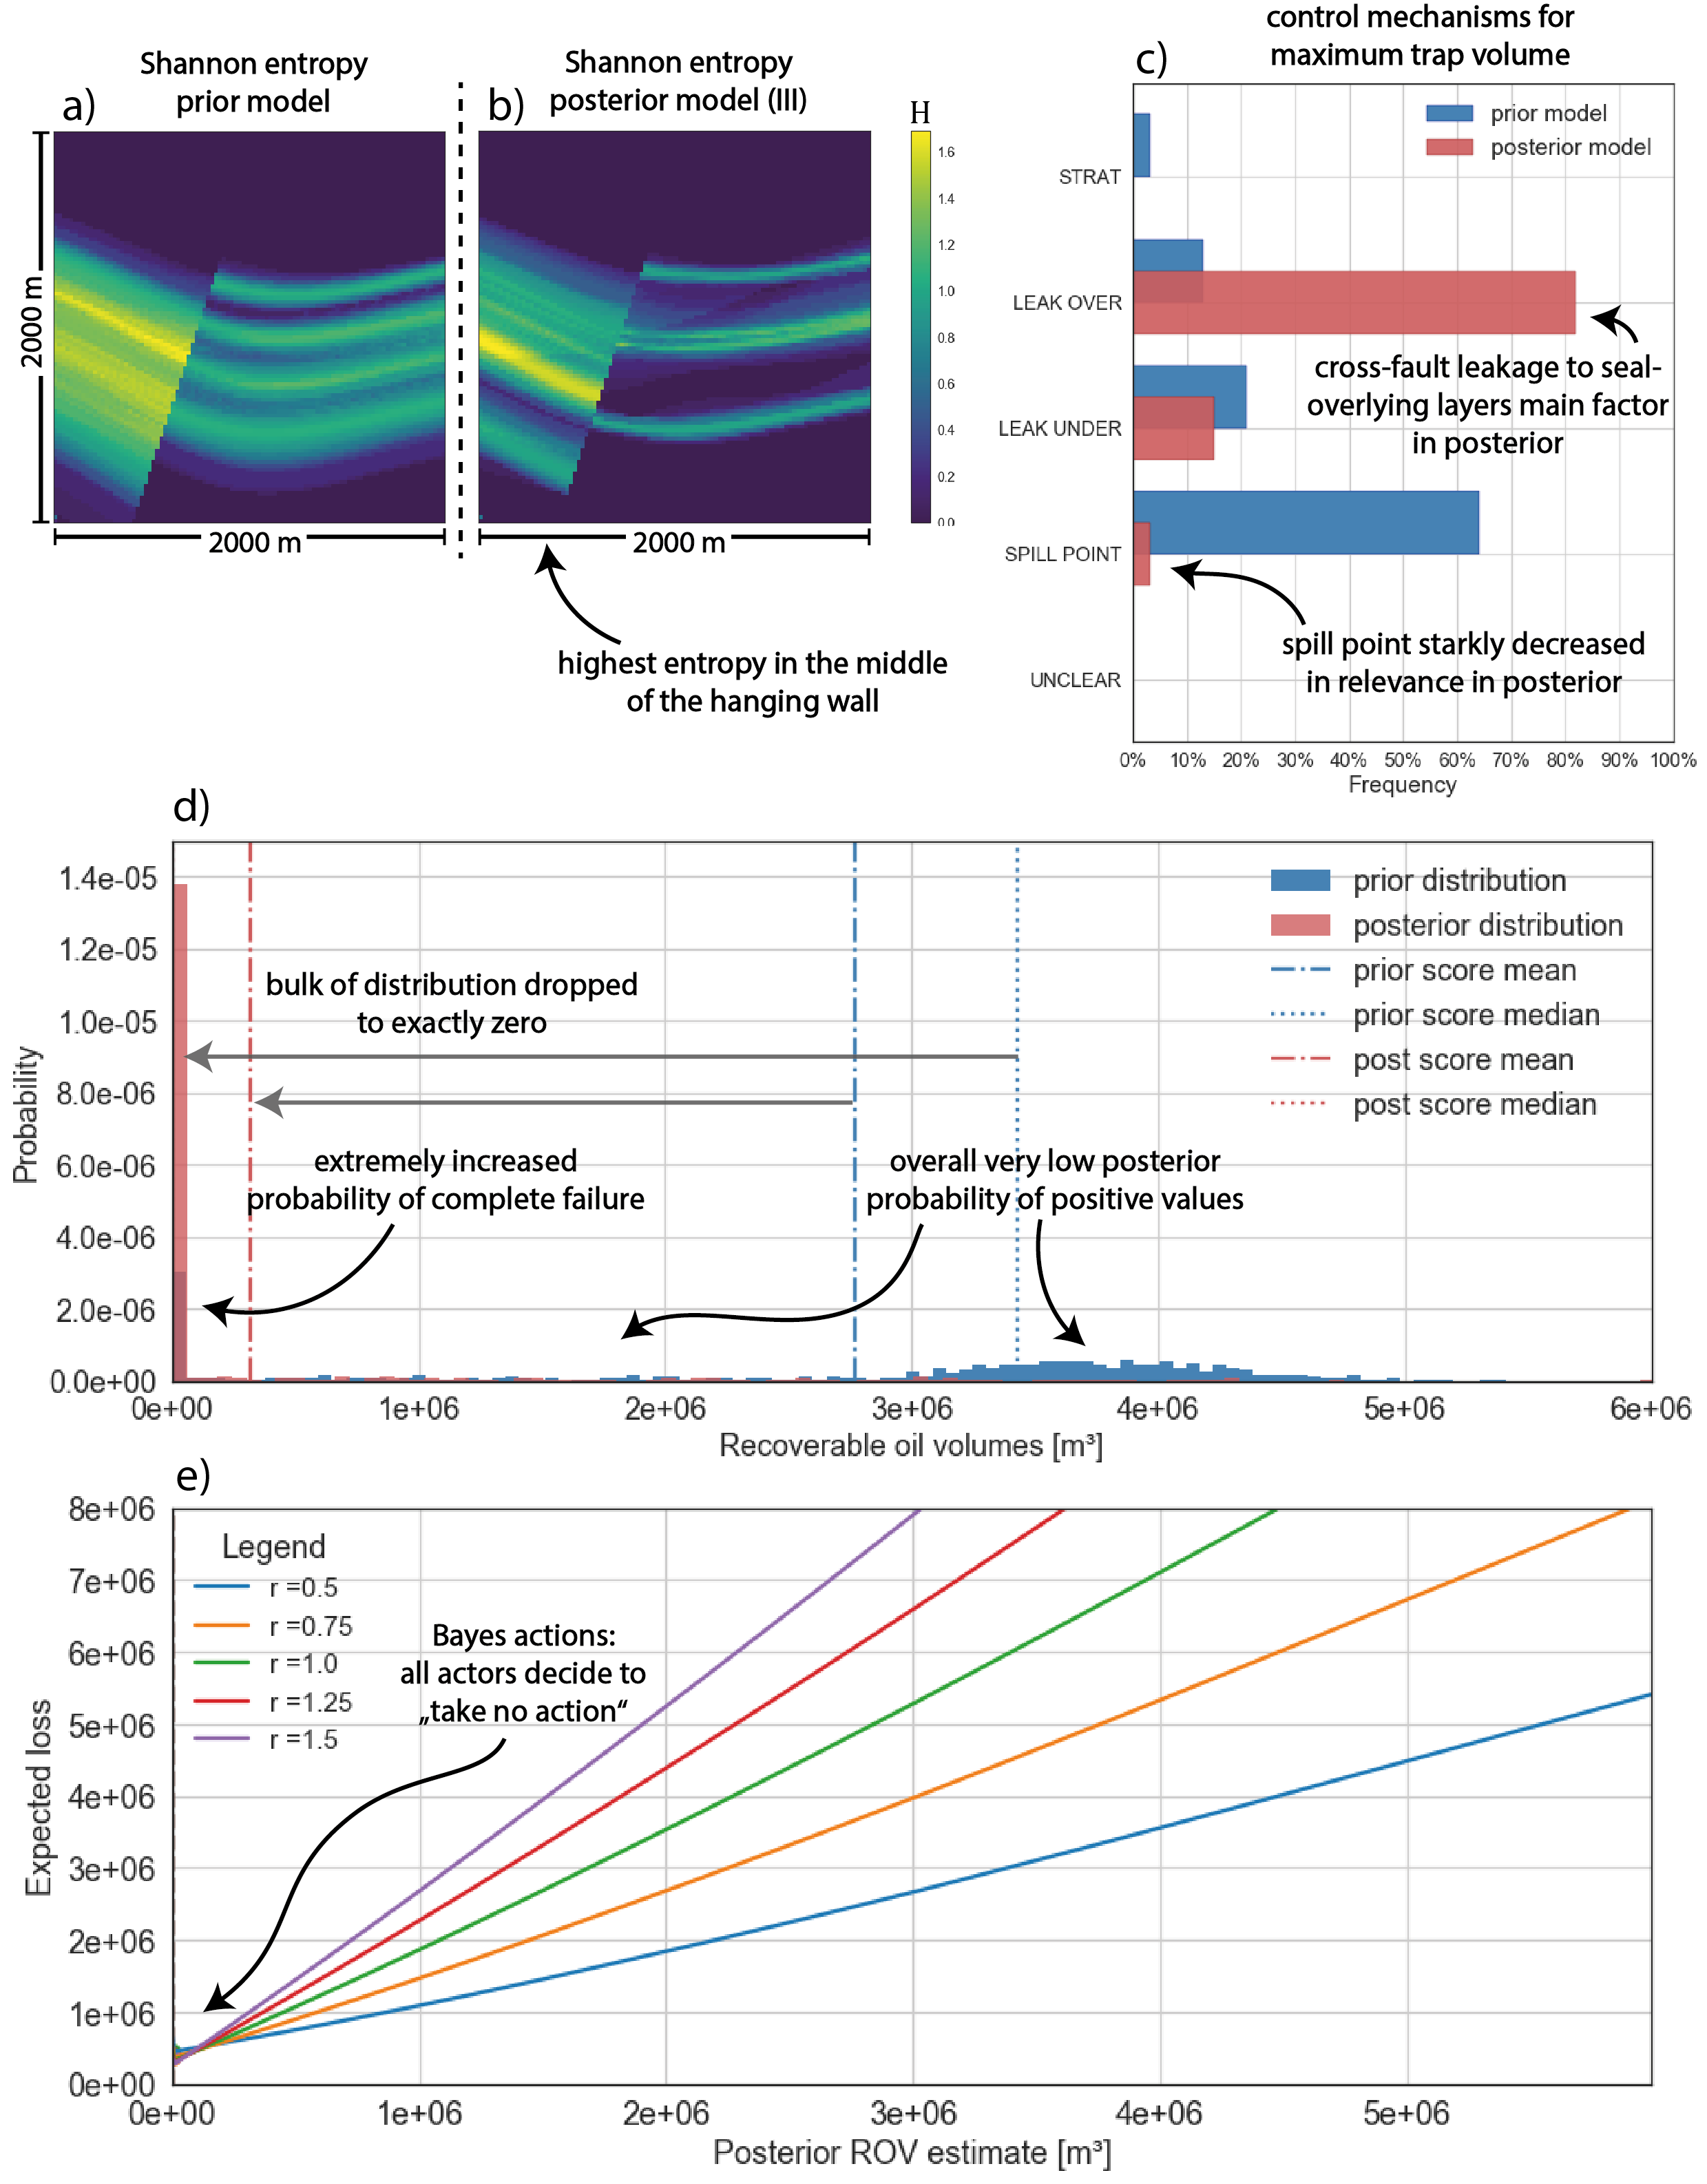
\includegraphics[width=1\textwidth]{Figures/ML2}
			\caption{Summary of results from evaluating posterior model III (3D). Shannon entropies in prior (a) and posterior (b) are compared. So are the mechanisms of maximum trap volume control (c). Prior and posterior ROV probability distributions are shown in (d). Respective loss function and Bayes actions are plotted in (e).}\label{fig:ML2}
		\end{figure}
		\begin{table}[h]
			\centering
			\begin{tabular}{lrr} 
				\toprule
				Model III - Likelihoods: layer thicknesses (normal distributions)\\  
				\midrule 
				Formation & $\mu$ [m] & $\sigma$ [m]\\ 
				\midrule 
				Sandstone 2 & 300 & 30 \\
				Shale (Seal) & 50 & 10\\ 
				Sandstone 1 (Reservoir) & 400 & 30 \\
				\bottomrule
			\end{tabular}
			\caption{Layer thickness likelihoods determined by normal distributions as used for posterior model III.}
			\label{tab:ML2_likelihoods}
		\end{table}
		Using likelihoods which favor a thick reservoir, but only a thin seal of about 50 m thickness (see Table \ref{tab:ML2_likelihoods}), leakage due to juxtaposition with seal-overlying formations across the fault ("LEAK OVER") became the primary mechanism for trap volume control (see Figure \ref{fig:ML2} (c). It can be recognized in Figure \ref{fig:ML2} (b) that, while uncertainty was reduced clearly in the footwall, it remained high in the hanging wall. The Shannon entropy visualization furthermore suggests that the seal layer frequently appeared significantly deeper in the hanging wall than in the footwall. Combined with a generally very thin seal, this allowed for the occurrence of high displacement to seal thickness ratios, i.e. a high SSF. Thus, frequent surpassing of the critical SSF and subsequent fault seal breaching were enabled. It is additionally apparent in Figure \ref{fig:ML2} (b), that while fault-related leakage became predominant, control by the spill point was suppressed to be widely irrelevant in this posterior model.\\	%It is suggested by the footwall information entropy in Figure \ref{label} (b), that the general shape of the structure has been flattened.
		A dramatically higher probability of complete trap failure was induced by the high frequency of cross-fault leakage to overlying formations. Consequently, the bulk of the posterior ROV probability distribution was shifted to a volume of zero, as depicted in Figure \ref{fig:ML2} (d). Any positive trap volumes have become highly improbable.\\
		Bayes actions changed accordingly. Given this posterior ROV distribution, all actors find their minimum of expected loss at ROV = 0, which equals the decision to "take no action" (see Figure \ref{fig:ML2} (e)). It has to be pointed out that all Bayes actions are found at the same point due to the lack of negative values into which more risk-averse actors would presumably have moved, given the possibility. This poses a difference to the score system implemented for the 1D geological model evaluation. As volumes cannot be negative, Bayes actions cannot be shifted past the limit of ROV = 0. Compared to the prior model, expected losses decreased overall, but are higher for risk-friendlier individuals at the minimum. Results from this third model show that in contrast to the reservoir thickness, seal thickness is a primary and decisive factor for the manifestation of a reliable trap structure.
		
		\subsection{3D - Posterior model IV: SSF likelihood reinforcing trap reliability}\label{sec:model4}%ML4
		\begin{figure}[p!]
			\centering
			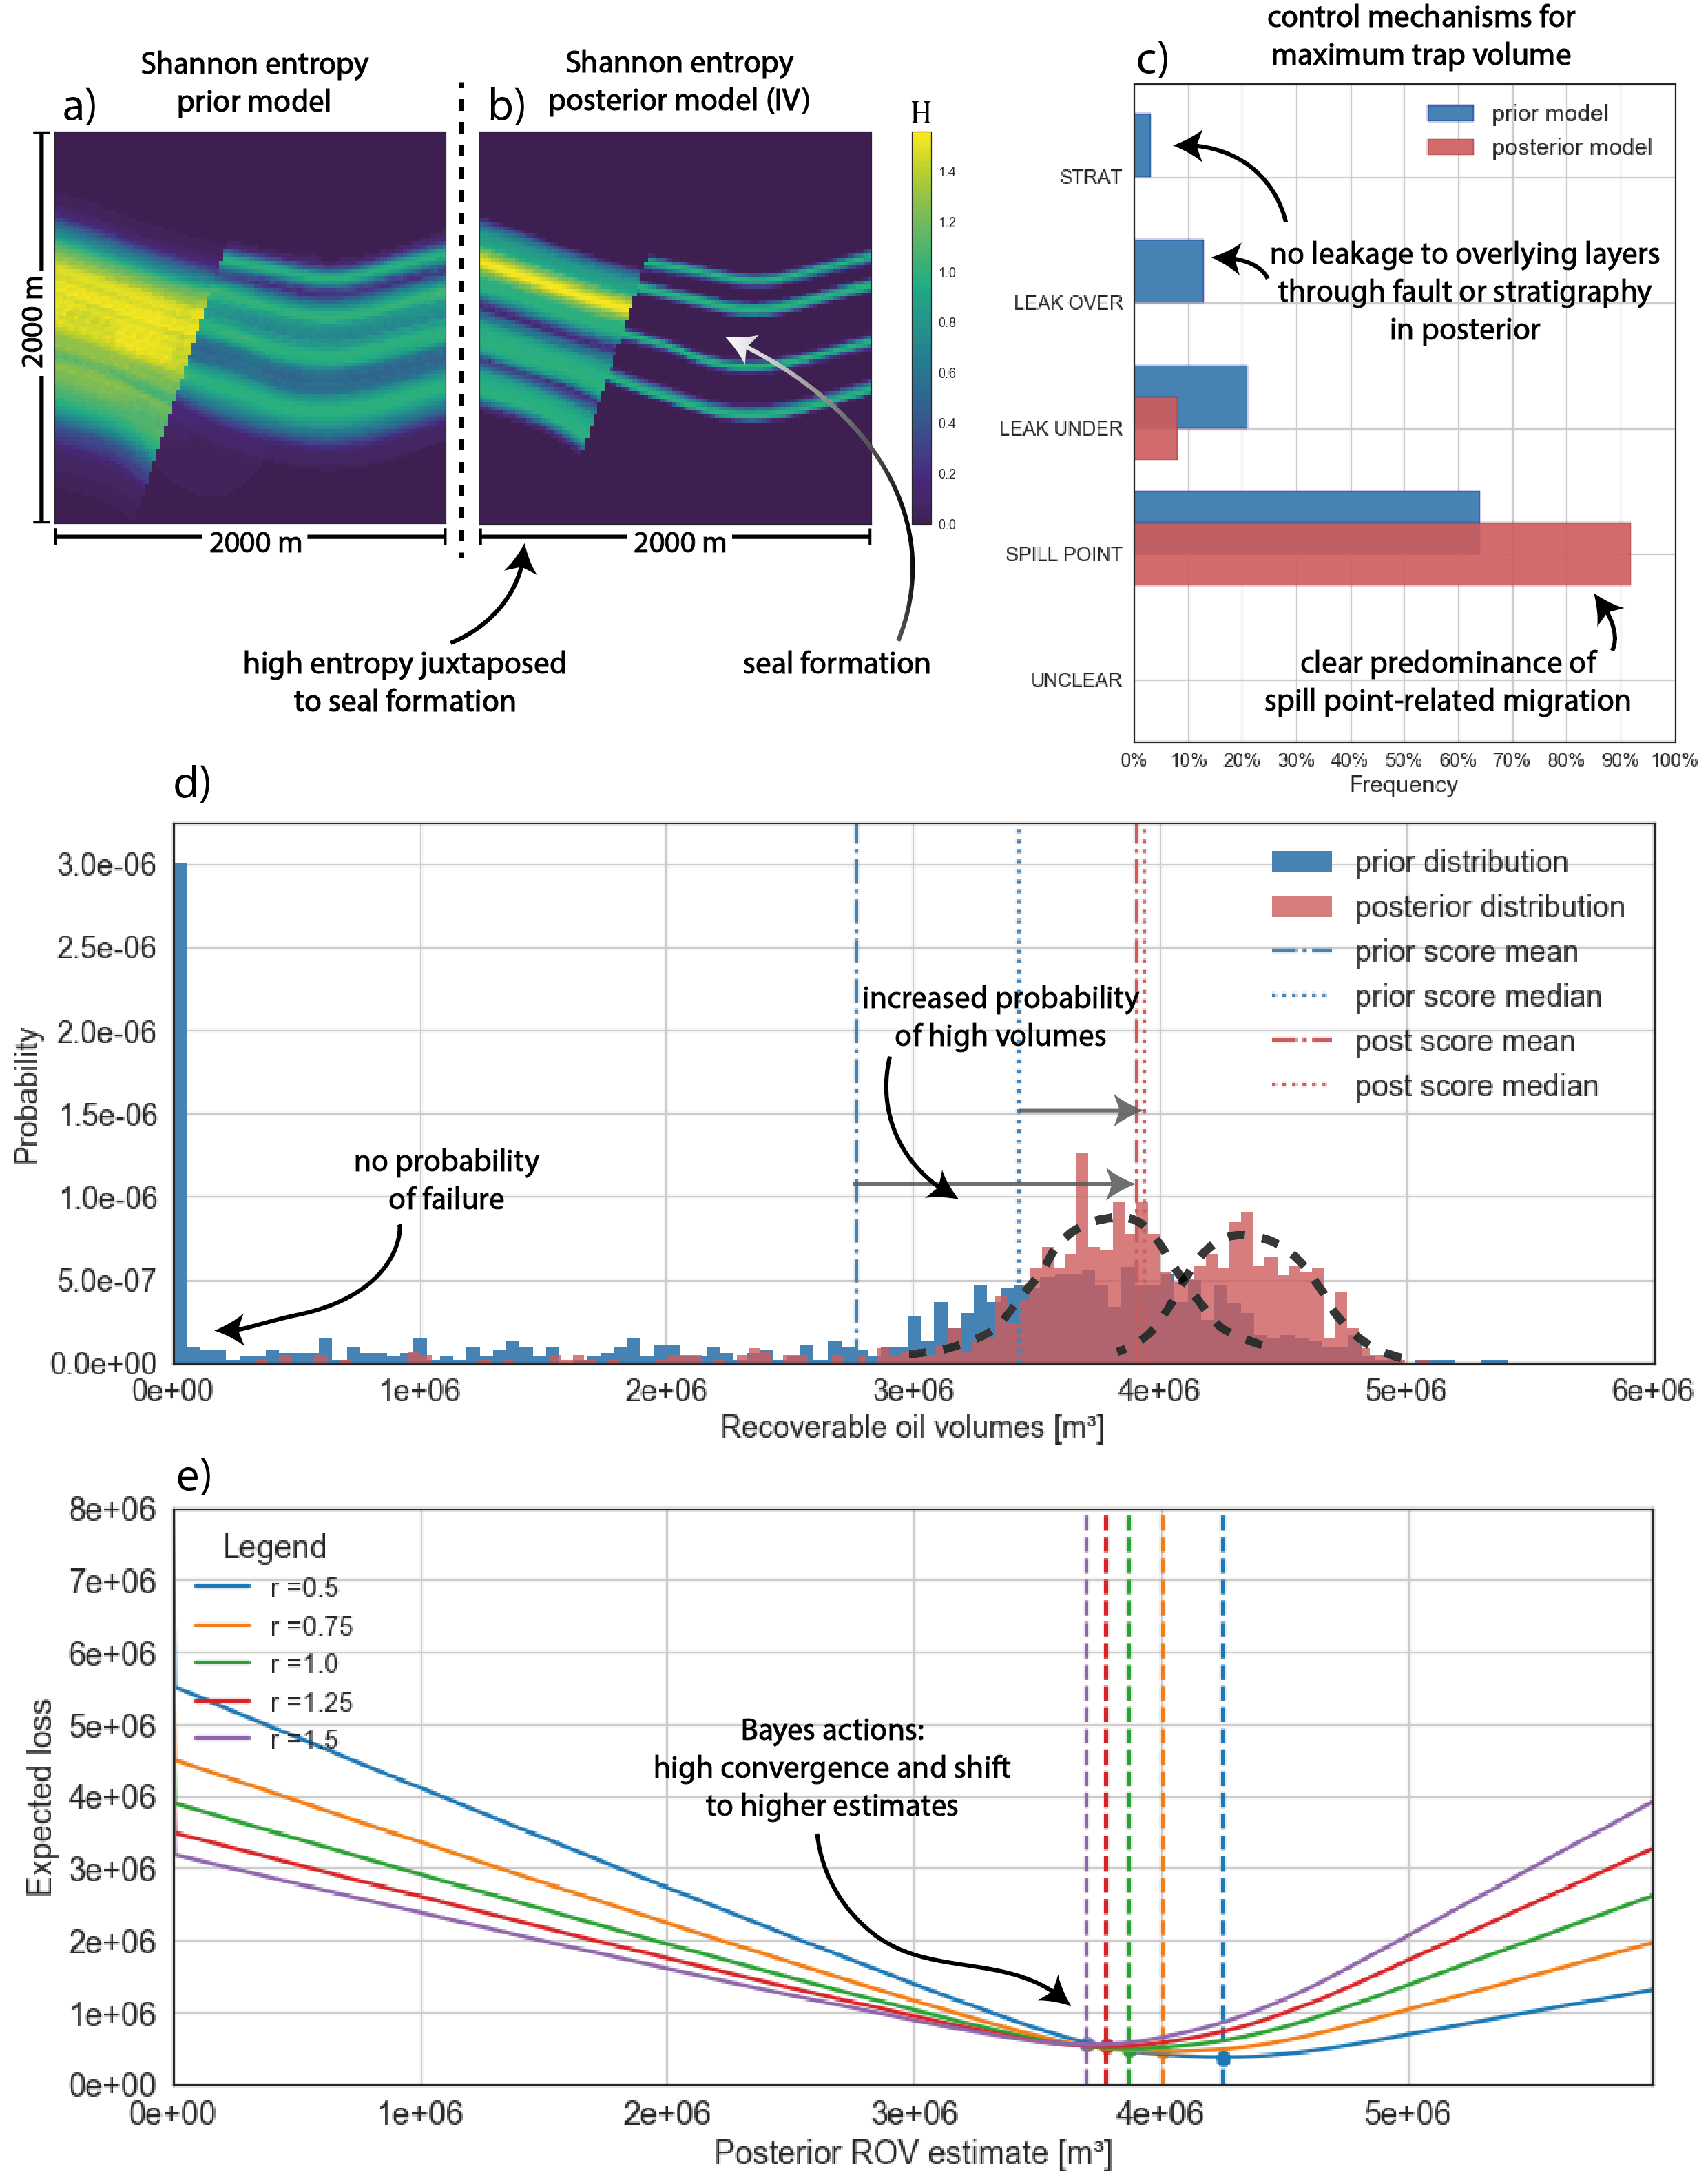
\includegraphics[width=1\textwidth]{Figures/Appendix/ML4}
			\caption{Summary of results from evaluating posterior model IV. Shannon entropies in prior (a) and posterior (b) are compared. So are the mechanisms of maximum trap volume control (c). Prior and posterior ROV probability distributions are shown in (d). Respective loss function and Bayes actions are plotted in (e).}\label{fig:ML4}
		\end{figure}
		\begin{table}[h]
			\centering
			\begin{tabular}{lrr} 
				\toprule
				Model IV - Likelihood: layer thicknesses (normal distributions)\\  
				\midrule 
				Formation & $\mu$ [m] & $\sigma$ [m]\\ 
				\midrule 
				Sandstone 2 & 150 & 20 \\
				Shale (Seal) & 300 & 30\\ 
				Sandstone 1 (Reservoir) & 250 & 25 \\
				\bottomrule
				\toprule
				Likelihood: Shale Smear Factor (normal distribution)\\
				\midrule
				- & $\mu$ & $\sigma$\\
				\midrule
				SSF & 1.5 & 0.5\\
				\bottomrule
			\end{tabular}
			\caption{Layer thickness likelihoods and SSF likelihood determined by normal distributions as used for posterior model IV (3D).}
			\label{tab:ML4_likelihoods}
		\end{table}
		For this fourth model, thickness likelihoods were chosen to be comparable to those of model I, i.e. supporting the probability of thick layers in general. Additionally, a SSF-related likelihood function was implemented. With a mean of 1.5 and a standard deviation of 0.5, it was chosen to mostly reinforce the likelihood of a SSF below the critical value of SSF$_\text{c} = 3$ (see Table \ref{tab:ML4_likelihoods}).\\
		In Figure \ref{fig:ML4} (b), it can be seen that the uncertainty about the position of interfaces in the footwall was greatly reduced for all layers. In the hanging wall, Sannon entropy remained higher but was shifted upwards and mainly concentrated in an area that is juxtaposed to the footwall seal formation.\\
		In the resulting ROV distribution, the possibility of trap failure was completely extinguished, while the probability of high volumes in the range between 3.5  and 5 million m$^3$ was significantly increased. Mean and median are found at almost the same value, but the bulk of the distribution found in this range appears to be slightly bimodal in itself, resembling approximately the shape of two normal distributions overlapping around the value of 4.3 million m$^3$.\\
		Accordingly, Bayes actions converged within this range of positive values. Considering the two modes in this range, risk-averse to risk-neutral bids remained in the middle of the mode of lower volumes, while the risk-friendliest actor was encouraged to bid on a higher volume found in the second mode. Overall, significant convergence was achieved, also in respect to expected losses.\\		
		The importance of a safe seal was once again emphasized by these results. Reliable fault sealing was favored by the chosen SSF likelihood. It should be pointed out that computation of the complete model is required to attain the SSF. This value is furthermore characterized by a complex interdependence with other parameters and is directly related to layer thicknesses and fault offset. For this reason, information entropy and offset uncertainty in the hanging wall were not greatly reduced. However, the certainty about the ratio of displacement to layer thicknesses was presumably improved by using the SSF in a likelihood function.
		
		\subsection{3D - Posterior model V: Controversial information about the Shale Smear Factor}\label{sec:model5}%ML5
		\begin{figure}[p!]
			\centering
			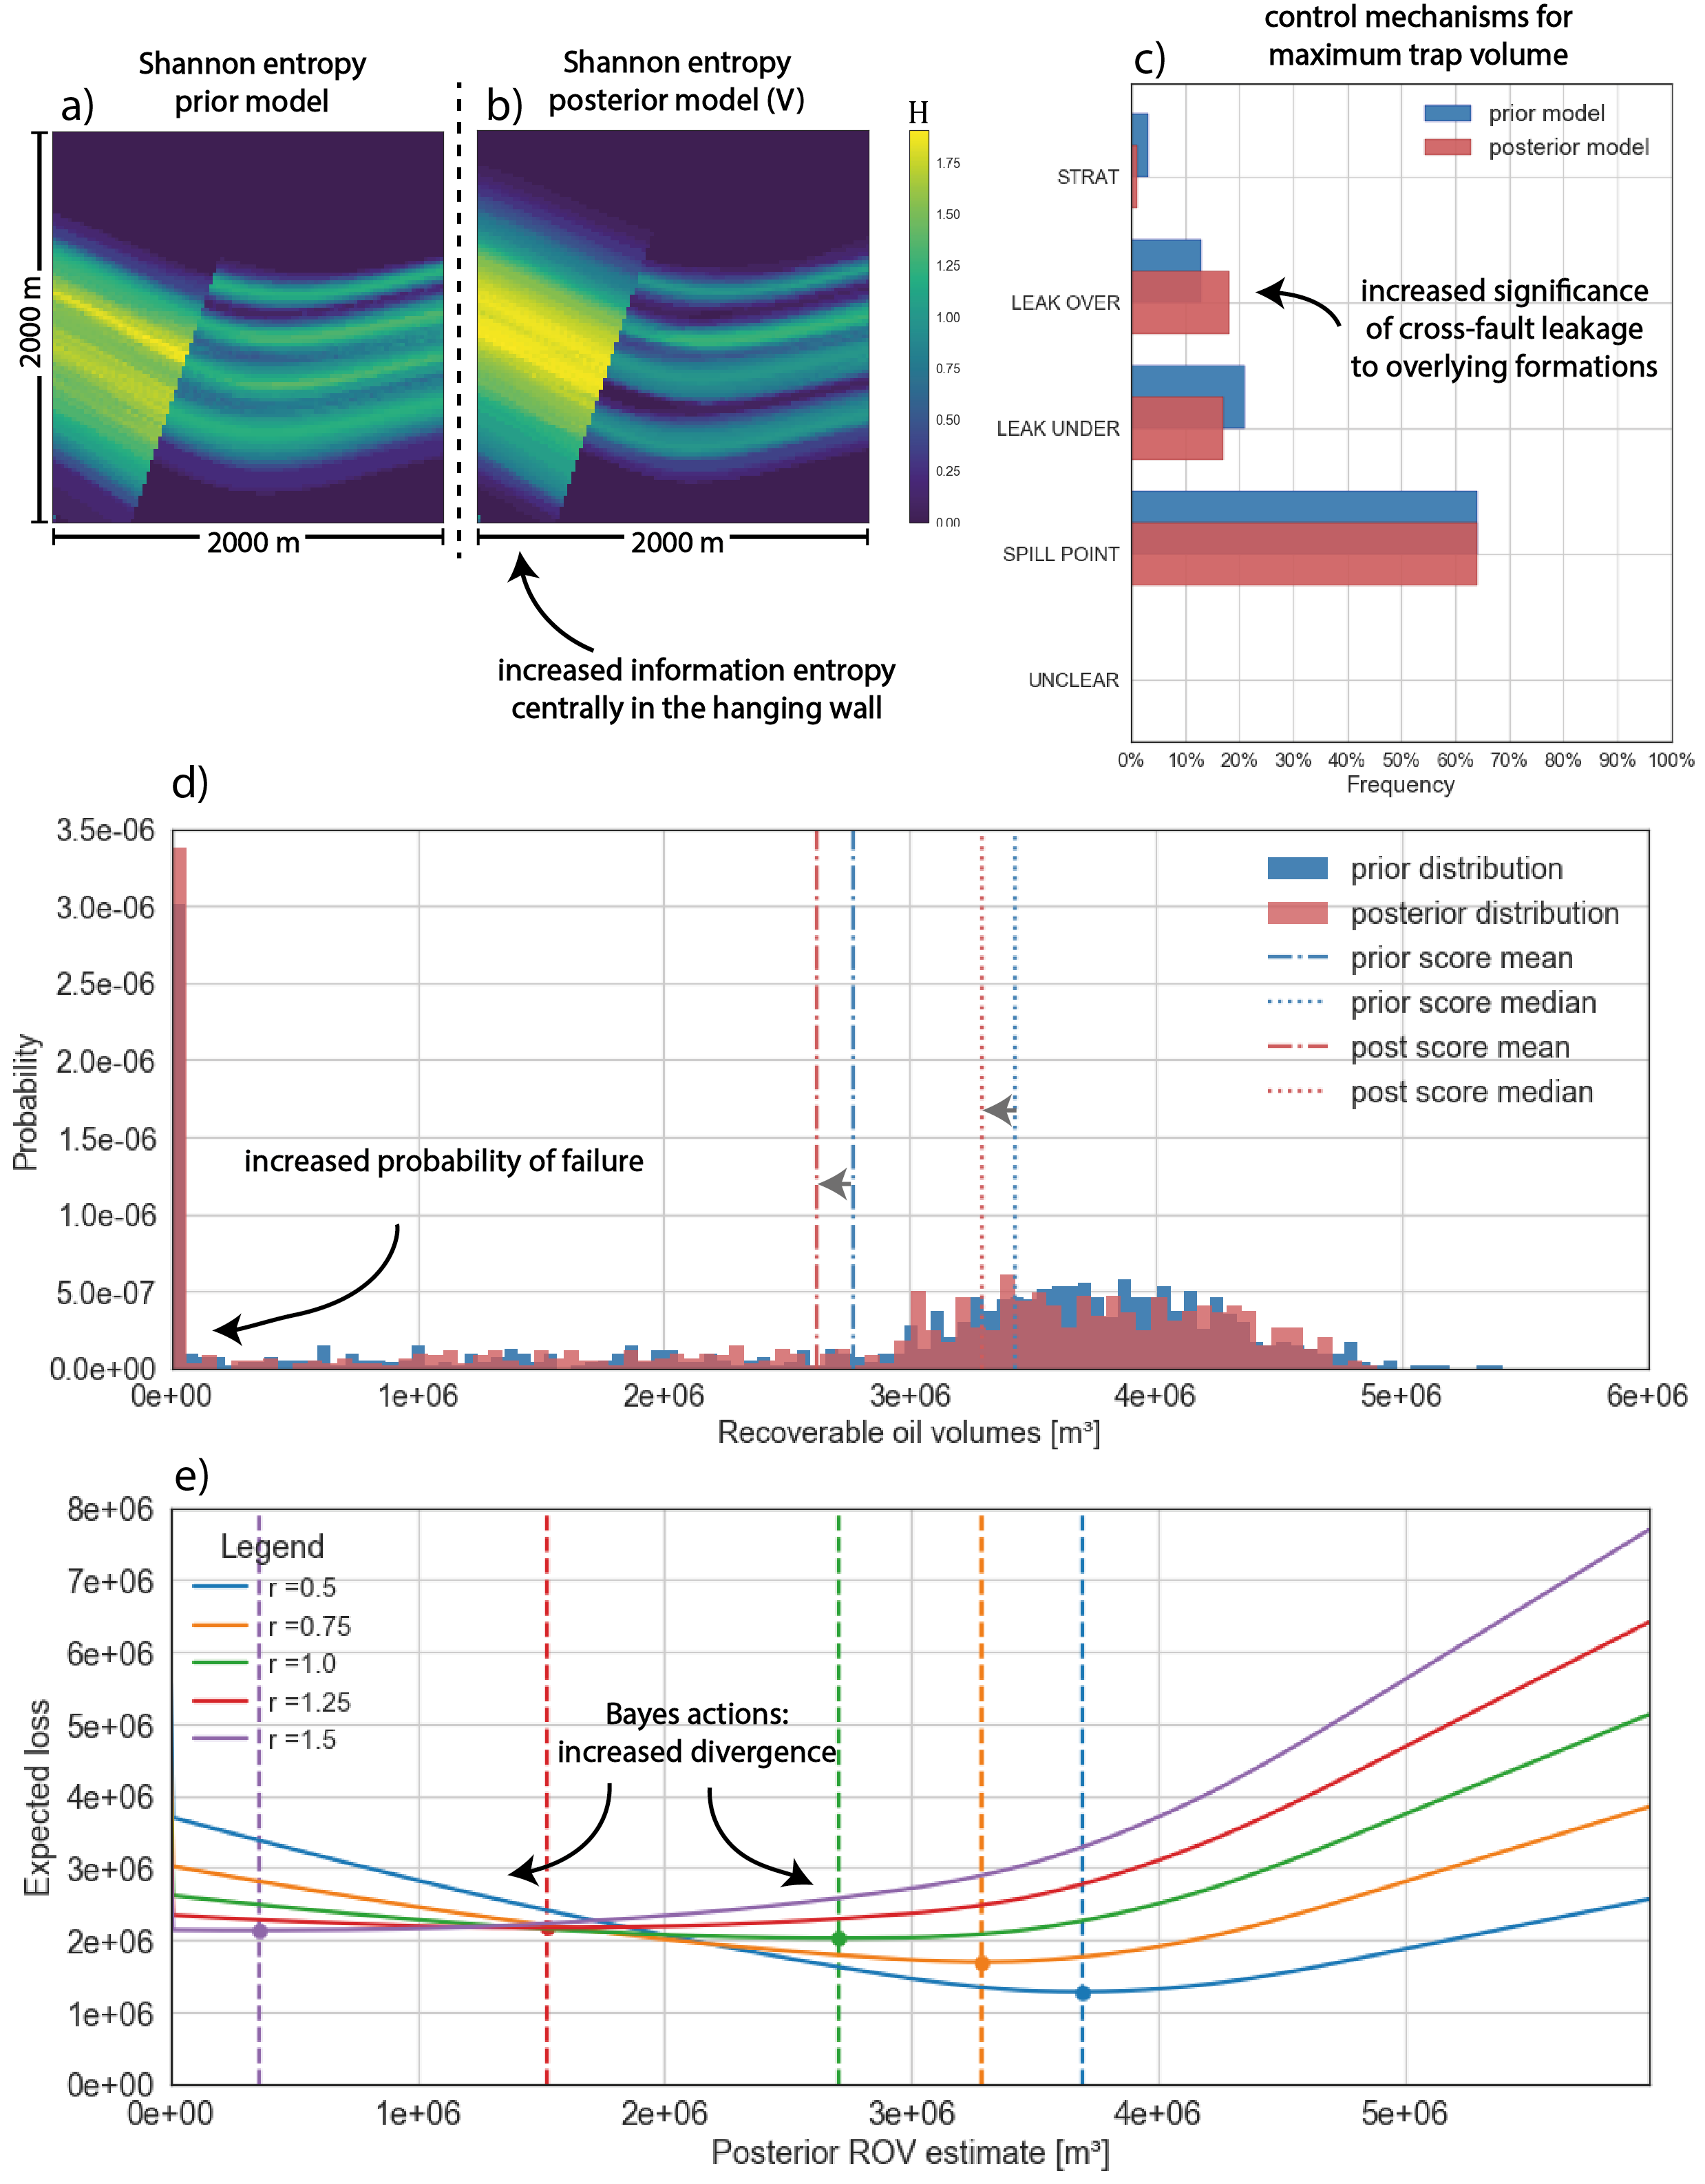
\includegraphics[width=1\textwidth]{Figures/ML5}
			\caption{Summary of results from evaluating posterior model V. Shannon entropies in prior (a) and posterior (b) are compared. So are the mechanisms of maximum trap volume control (c). Prior and posterior ROV probability distributions are shown in (d). Respective loss function and Bayes actions are plotted in (e).}\label{fig:ML5}
		\end{figure}
		\begin{table}[h]
			\centering
			\begin{tabular}{lrr} 
				\toprule
				Model V - Likelihood: Shale Smear Factor (normal distribution)\\
				\midrule
				- & $\mu$ & $\sigma$\\
				\midrule
				SSF & 3 & 0.3\\
				\bottomrule
			\end{tabular}
			\caption{SSF likelihood determined by a normal distributions as used for posterior model V (3D).}
			\label{tab:ML5_likelihoods}
		\end{table}
		In this last case example, no thickness likelihoods, only a SSF-related likelihood was used. In contrast to model IV, this was chosen to narrow the probability of the SSF to be around the threshold of its critical value of SSF$_\text{c} = 3$ (see Table \ref{tab:ML5_likelihoods}).\\
		Results are relatively similar to those of the prior model. Shannon entropies were only slightly decreased overall (Figure \ref{fig:ML5} (b)). An increase in the relevance of cross-fault leakage to overlying formations ("LEAK OVER") as a trap volume mechanism (increase from $\sim13\%$ to $\sim18\%$) was observed (Figure \ref{fig:ML5} (c)). Consequently, the bimodal character between the bulk of positive values and the probability of complete failure in the ROV distribution was reinforced. This is also indicated by a shift of mean and median to lower volumes (Figure \ref{fig:ML5} (d)). Accordingly, a higher degree of decision divergence, i.e. a greater separation of different Bayes actions, was induced (Figure \ref{fig:ML5} (e)). Expected losses of these minima were raised as well.\\
		It is notable that the implementation of a likelihood function, which can be expected to significantly decrease the SSF related uncertainty, overall leads to an amplification of the duality in the ROV probability distribution and to dispersion of differently risk-affine decisions. This effect is presumably caused by conservation of decisive uncertainty between "success" and complete failure of the trap, due to narrowing of the SSF probability around its critical value. 